% stato della relazione :
%
%AMMERDAAAAAAAA
%
\documentclass[a4paper,twoside]{article}

\usepackage[margin=3cm]{geometry}
\usepackage[utf8]{inputenc}
\usepackage[main=italian, english]{babel}
\usepackage{graphicx}
\usepackage{rotating}
\usepackage{verbatim}
\usepackage{listings}
\usepackage[colorlinks=true,linkcolor=black,urlcolor=blue]{hyperref} % ancore delle varie sezioni sul menu
\usepackage{float}
\graphicspath{ {Immagini-Grafici/} }

\author{Giuseppe Merlino, Miki Violetto}
\title{Relazione progetto BiciRent}
\date{\today}

\begin{document}
\maketitle

\newpage
\tableofcontents
\newpage
\listoffigures
\newpage

\section{Abstract}
BiciRent è un servizio di bike sharing ispirato a Goodbike presente qui a Padova.\newline
Permette il noleggio di biciclette da utilizzare per girare in città grazie a tessere personali e molte stazioni dislocate su varie aree della città è possibile prelevare e depositare la bicicletta con comodità.\newline
Il progetto si focalizza sulla gestione dei noleggi e delle operazioni di routine eseguibili dall'utenza e dai tecnici di BiciRent, virtualizzando su un sito le operazioni che verrebbero normalmente svolte su vari dispositivi come le colonnine, un'applicazione per gli utenti o una per i tecnici.
\section{Descrizione testuale dei requisiti e operazioni tipiche}
\subsection{Descrizione testuale}
Al momento dell'iscrizione di un utente verranno richiesti tutti i dati personali necessari a registrarlo e rilasciarli la tessera, quali nome, cognome, data e luogo di nascita, informazioni sulla residenza, e un'email quale recapito per essere contattato; grazie a queste informazioni gli verrà rilasciata una tessera personale con la quale utilizzare tutti i servizi, e avente una data di attivazione.\newline
Bisognerà registrare se l'utente è un turista o uno studente, i quali però dovranno dimostrare di esserlo con la matricola universitaria o la carta IoStudio; il sito svolge solo un'azione di deposito dei dati.\newline
Un utente potrà quindi prelevare una bicicletta da una colonnina di una stazione e poi depositarla su una qualsiasi colonnina libera: queste operazioni, chiamate prelievo e deposito, dovranno venire registrate dal sito con in aggiunta l'orario in cui vengono effettuate.\newline
Sia le biciclette che le colonnine sono dei beni identificati da un codice comune che identifica tutti i beni dell'azienda BiciRent, inoltre questi materiali possono essere danneggiati: un materiale danneggiato non permette alcuna operazione su di esso da parte dell'utente e deve venire riparato dai tecnici.\newline
Deve venire registrata ogni riparazione eseguita dai tecnici, con in aggiunta una descrizione del danno riparato.\newline
Le biciclette possono essere a pedalata assistita (elettriche) oppure normali e possono essere in servizio (cioè ferme nelle colonnine oppure noleggiate) o in magazzino; una bicicletta danneggiata può ovviamente essere collegata ad una colonnina o in magazzino.\newline
Le colonnine sono presenti in gruppi su tutto il territorio, raggruppate in stazioni che vengono identificate dal loro indirizzo, e possono essere libere oppure occupate da una bicicletta. La colonnina segnalata rende danneggiata anche la bicicletta, se presente.\newline
Ulteriori informazioni che devono essere registrate sono le segnalazioni da parte dell'utente e le informazioni relative ai trasporti eseguiti dai tecnici.\newline
Un utente può segnalare la mancanza in una stazione, cioè se vuole eseguire un noleggio (o un deposito) e la stazione ha tutte le colonnine vuote (o occupate) può segnalare questo ai tecnici; oltre alla  rottura di una colonnina ( e quindi della bicicletta collegata).\newline
I trasporti eseguiti dai tecnici sono del tutto simili alle operazioni eseguite dai clienti, solo che l'aggiunta o rimozione di una bicicletta può essere eseguita solo dai tecnici, mentre il noleggio e il deposito solo dai clienti muniti di tessera, ma non si vuole tener traccia del tecnico.\newline
Il sito dovrà virtualizzare le operazioni che normalmente un cliente esegue su una colonnina, quindi un prelievo di una bicicletta passando la sua tessera, o un deposito, o una segnalazione di rottura (eseguita su una colonnina, per questo non si discrimina se è la bicicletta o la colonnina); dovrà inoltre prevedere un'area in cui è possibile per l'utente controllare i suoi noleggi, i suoi dati personali e lo stato delle stazioni ( nella realtà queste informazioni gli sono accessibili tramite un'applicazione per smartphone). Inoltre dovrà esserci un'area amministrativa in cui i tecnici possono registrare le manutenzioni che fanno e controllare le segnalazioni eseguite dagli utenti.\newline
Alcune informazioni di traffico previsto: si prospettano circa 1700 noleggi giornalieri e una media di 200 richieste d'intervento al giorno (mancanza di bici e rotture); inoltre viene richiesta la composizione dei posti delle stazioni (presenza biciclette, tipi disponibili e posti liberi) almeno 10000 volte ogni giorno, ma con punte di quasi 900 richieste in una singola mezz'ora (ad esempio nelle ore di punta).
\section{Progettazione concettuale}
Per la modellazione concettuale si è deciso di utilizzare un metodo misto e partire dall'operazione di noleggio.
\subsection{Noleggio}
Il noleggio è formato da due distinte operazioni, un prelievo che inizia il noleggio, e un deposito che lo termina.
\begin{figure}[h]
 \centering
 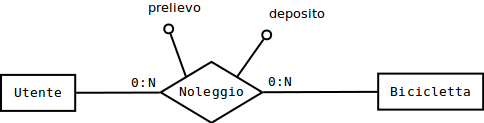
\includegraphics[width=0.7\textwidth]{Concettuale01}
\caption{Relazione Noleggio}
\end{figure}
\subsection{Utente}
Le informazioni personali dell'utente vengono rappresentate con l'entità Utente; Studente e Turista sono specializzazioni parziali esclusive; l'utente viene identificato dalla tessera che possiede e utilizza nel sito.
\begin{figure}[H]
 \centering
  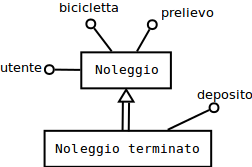
\includegraphics[width=0.6\textwidth]{Concettuale02}
\caption{Entità utente}
\end{figure}
\begin{figure}[H]
 \centering
  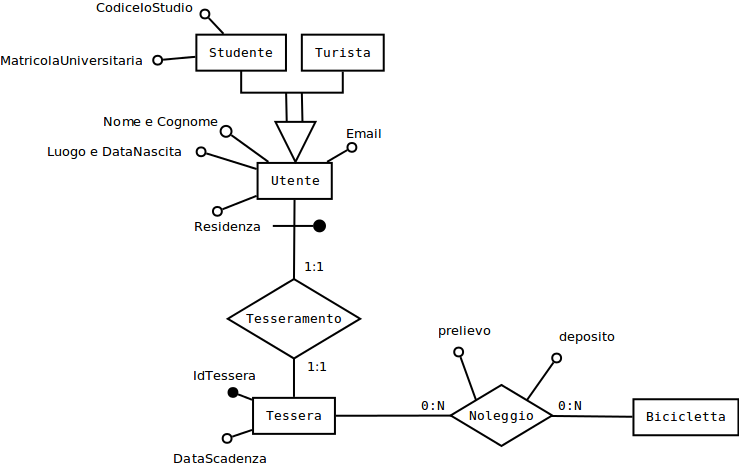
\includegraphics[width=1\textwidth]{Concettuale03}
\caption{Relazione Noleggio}
\end{figure}
\subsection{Tessera}
La informazioni di tessera non possono essere rappresentate da un singolo attributo, quindi lo si reifica in un'entità.
\begin{figure}[H]
 \centering
  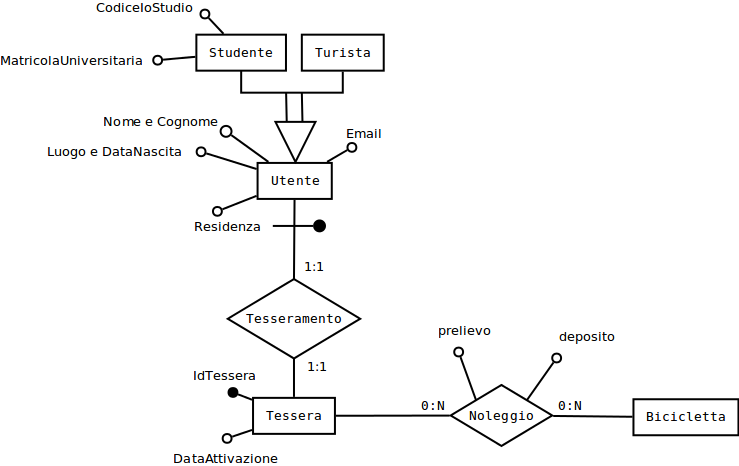
\includegraphics[width=1\textwidth]{Concettuale04}
\caption{Entità Tessera}
\end{figure}
\subsection{Bicicletta}
Le informazioni della bici vengono rappresentate dall'entità Bicicletta, identificata dal codice del materiale.
\begin{figure}[H]
 \centering
  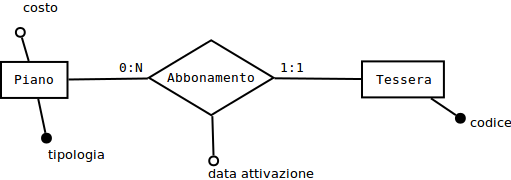
\includegraphics[width=1\textwidth]{Concettuale05}
\caption{Entità Bicicletta}
\end{figure}
\subsection{Operazione}
Sia prelievo che deposito sono operazioni con attributi propri.
\begin{figure}[H]
 \centering
  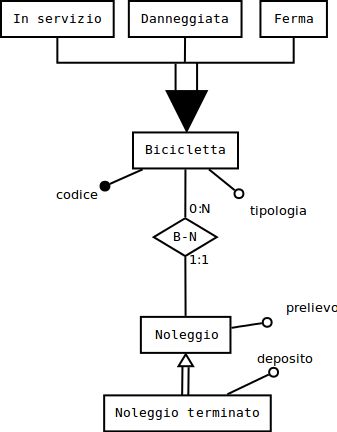
\includegraphics[width=0.3\textwidth]{Concettuale06}
\caption{Entità Operazione}
\end{figure}
\subsubsection{Eliminazione Noleggio}
Quindi la relazione noleggio scompare, essendo divisa in due relazioni che legano Tessera ad Operazione. Operazione inoltre contiene operazioni di trasporto.
\begin{figure}[H]
 \centering
  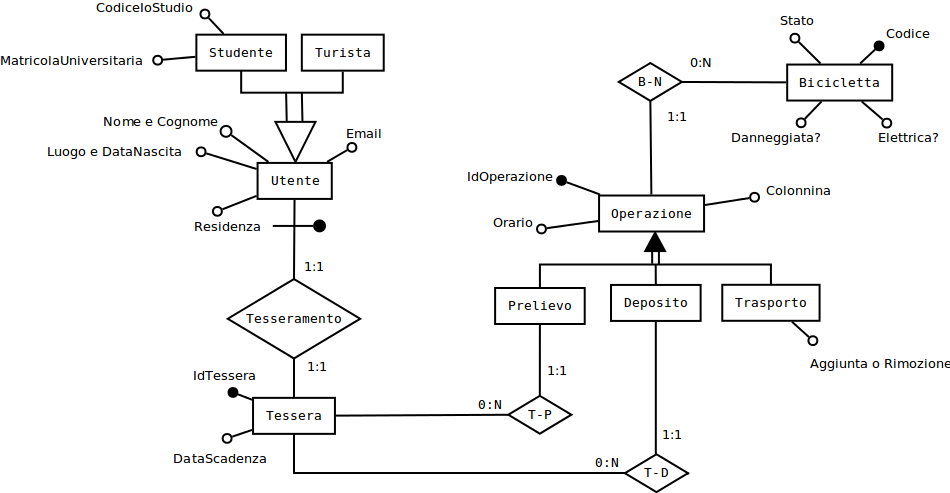
\includegraphics[width=1\textwidth]{Concettuale07}
\caption{Scomparsa della relazione Noleggio}
\end{figure}
\subsection{Colonnina}
La colonnina non può essere rappresentata da un solo attributo.
\begin{figure}[H]
 \centering
  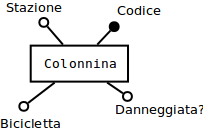
\includegraphics[width=0.3\textwidth]{Concettuale08}
\caption{Entità Colonnina}
\end{figure}
Per rappresentare la posizione di una Bicicletta su una Colonnina si utilizza una relazione.
\begin{figure}[H]
 \centering
  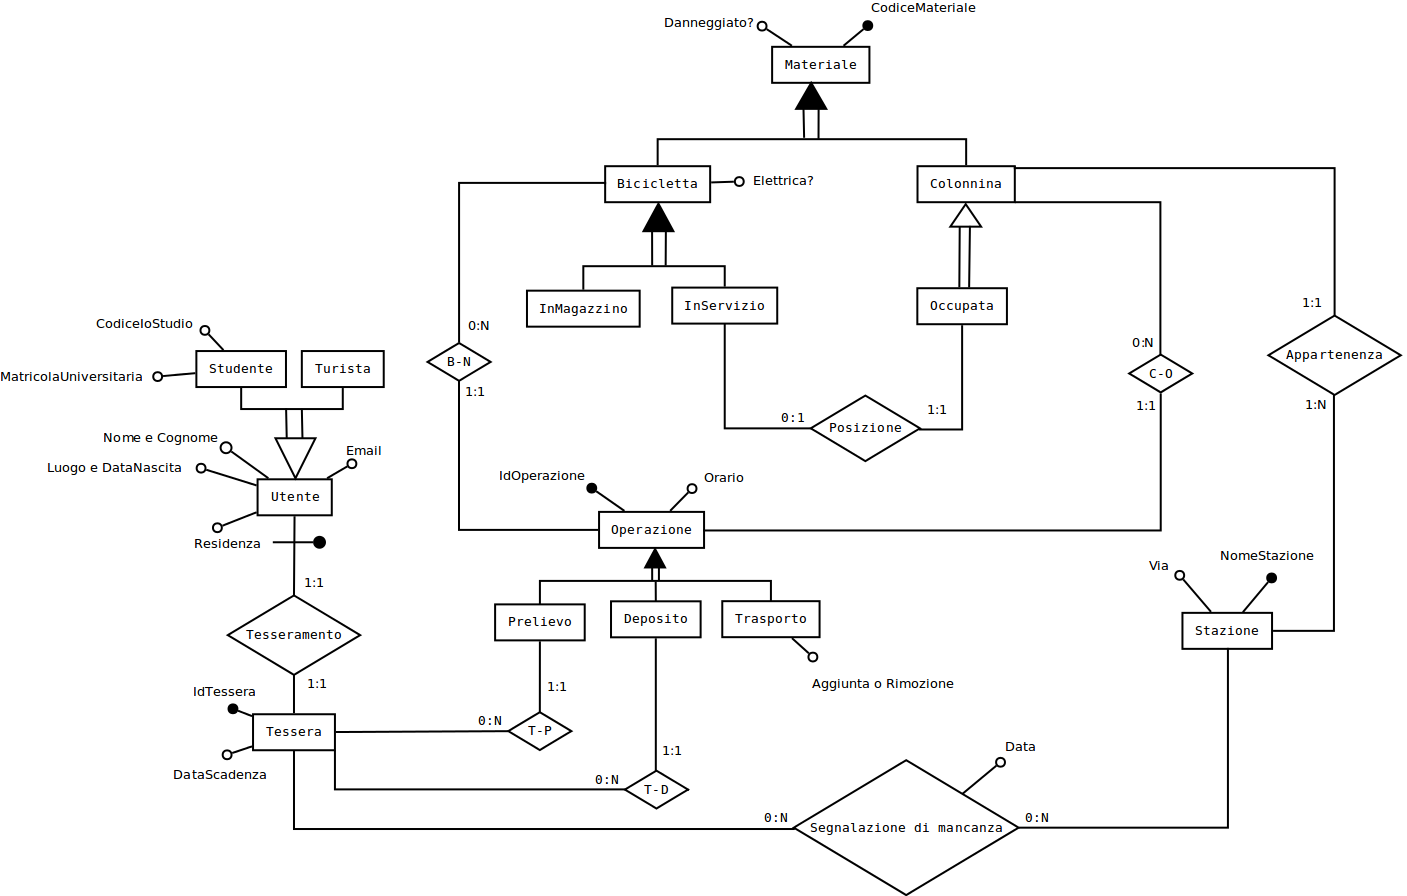
\includegraphics[width=0.7\textwidth]{Concettuale09}
\caption{Relazione Posizione}
\end{figure}
Quindi lo schema tra Operazione, Bicicletta e Colonnna è il seguente.
\begin{figure}[H]
 \centering
  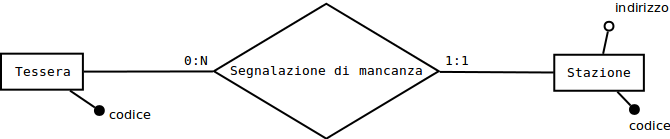
\includegraphics[width=1\textwidth]{Concettuale10}
\caption{Operazione, Bicicletta, Colonnina}
\end{figure}
\subsection{Stazione}
Le colonnine sono raggruppate in Stazioni.
\begin{figure}[H]
 \centering
  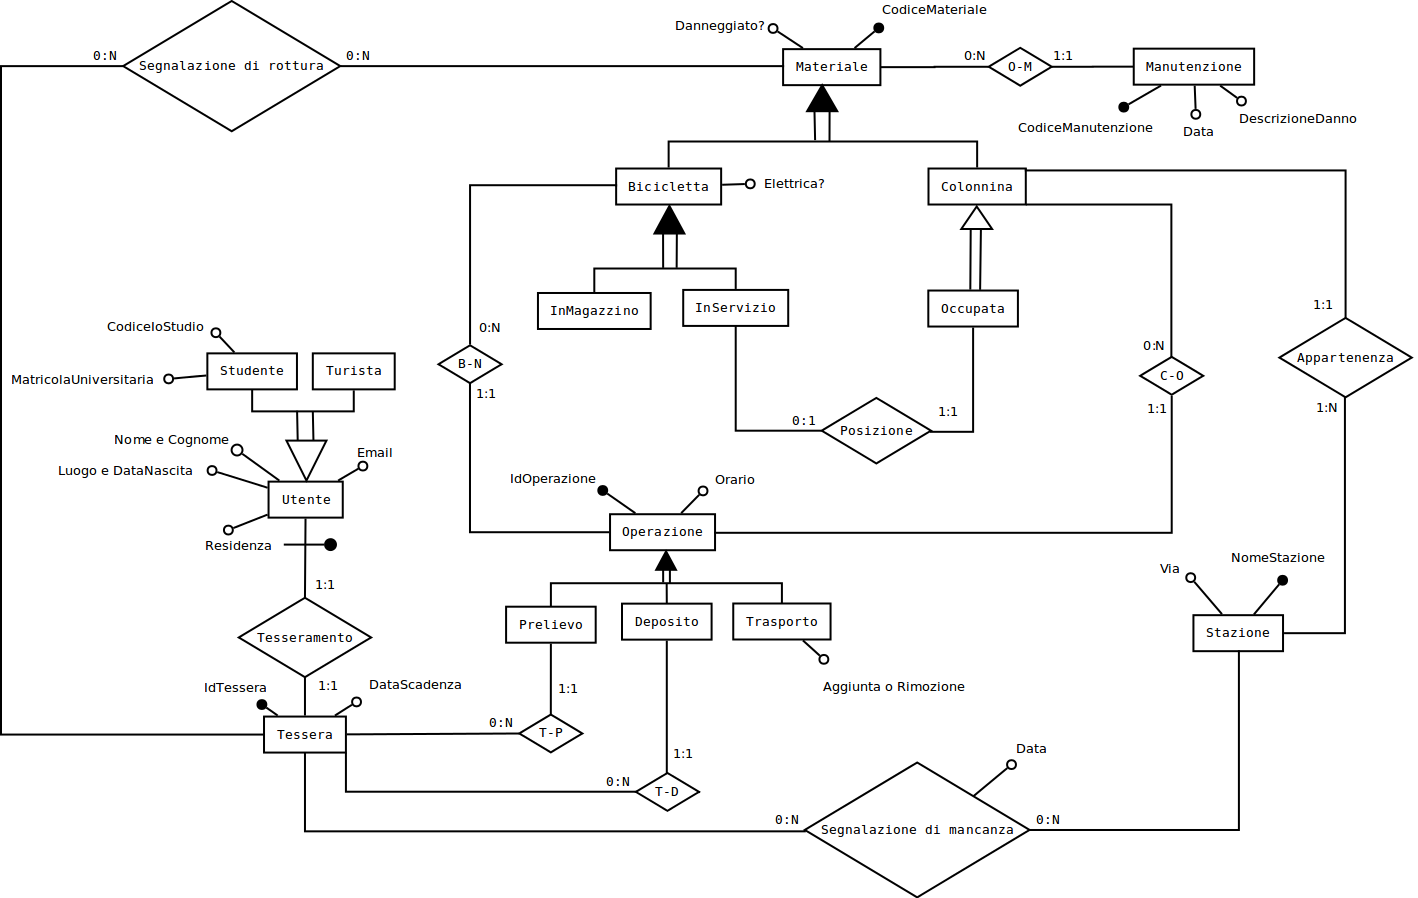
\includegraphics[width=0.6\textwidth]{Concettuale11}
\caption{Entità Stazione}
\end{figure}
\subsection{Materiale}
Come descritto dai requisiti, sia le Colonnine che le Biciclette sono dei materiali, quindi sono specializzazioni complete ed esclusive
\begin{figure}[H]
 \centering
  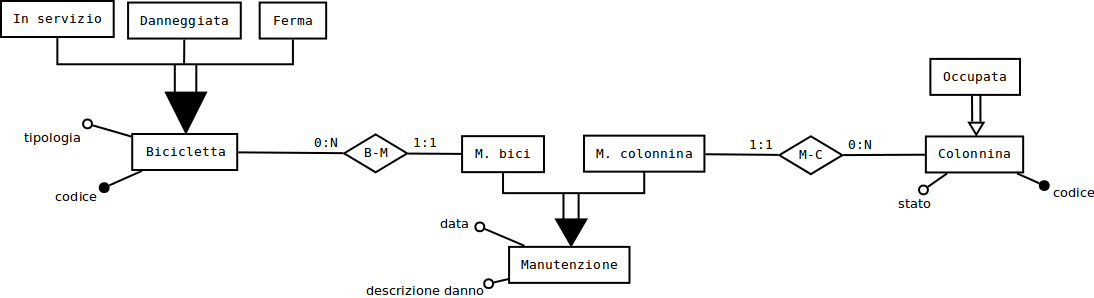
\includegraphics[width=0.6\textwidth]{Concettuale12}
\caption{Entità Materiale}
\end{figure}
\begin{figure}[H]
 \centering
  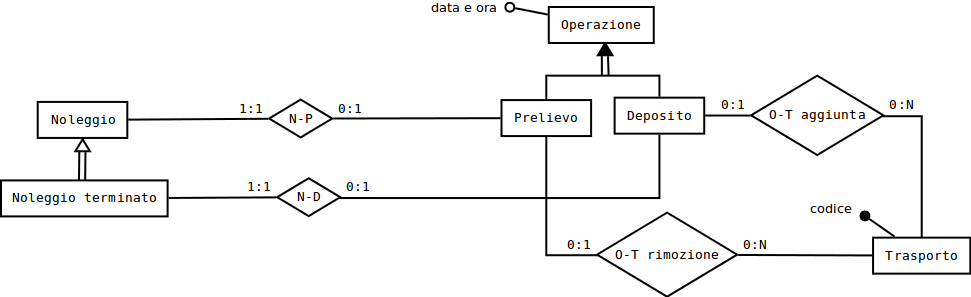
\includegraphics[width=1\textwidth]{Concettuale13}
\caption{Stato dell'Entità Materiale}
\end{figure}
\subsection{Segnalazioni}
Le segnalazioni di mancanza e rottura vengono realizzate tramite delle relazioni.
\begin{figure}[H]
 \centering
  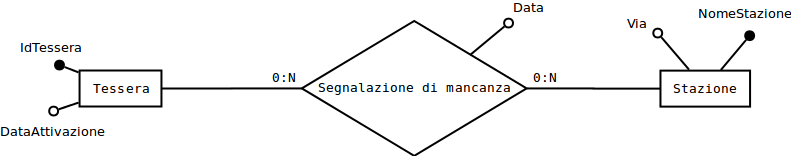
\includegraphics[width=1\textwidth]{Concettuale14}
\caption{Relazione Segnalazione di Mancanza}
\end{figure}
\begin{figure}[H]
 \centering
  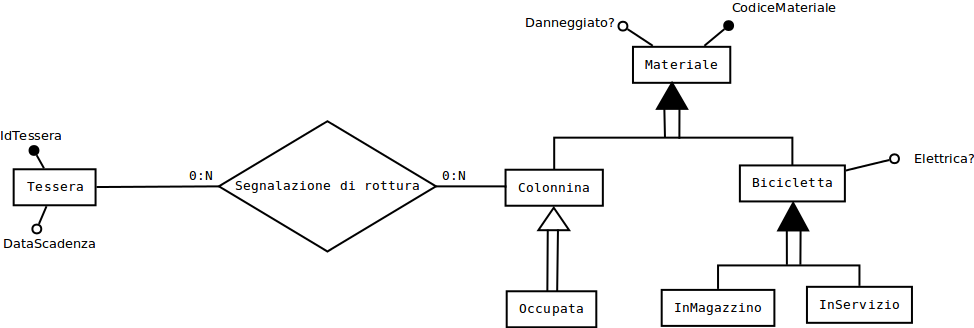
\includegraphics[width=1\textwidth]{Concettuale15}
\caption{Relazione Segnalazione di Rottura}
\end{figure}
\newpage
\subsection{Modello concettuale finale}
Questo è il modello concettuale risultante.
\begin{figure}[H]
 \centering
  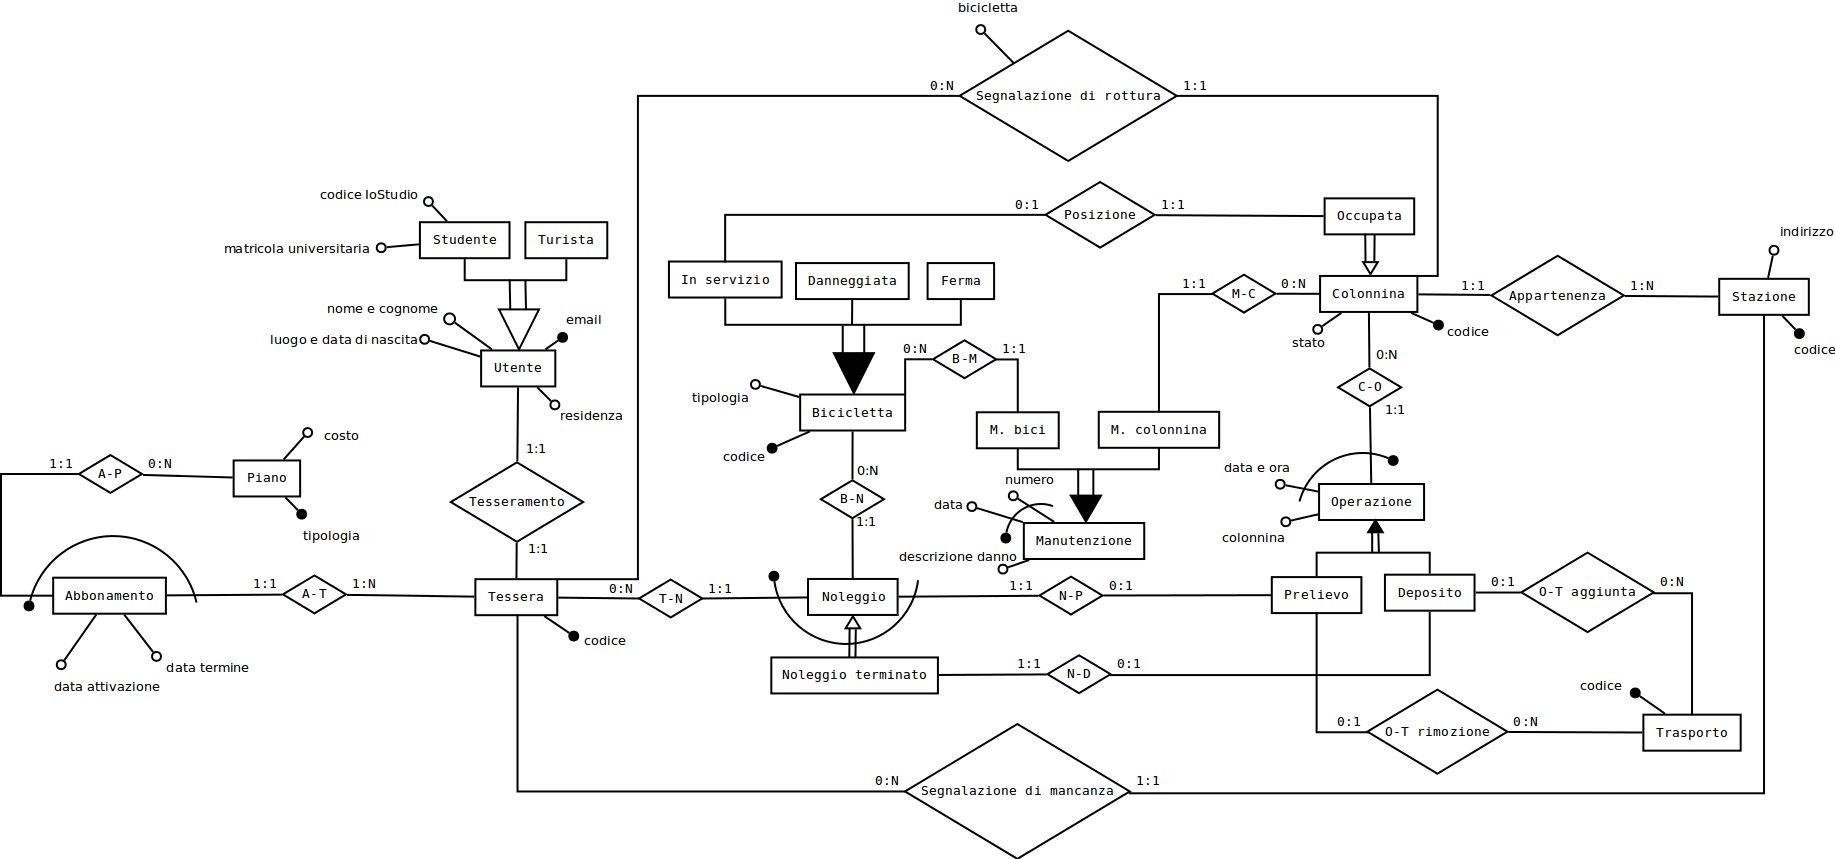
\includegraphics[width=1.35\textwidth,angle=90]{ConcettualeFinale}
\caption{Modello Concettuale Finale}
\end{figure}
\newpage
\section{Progettazione logica}
Per realizzare il modello logico siamo partiti da quello concettuale ed abbiamo controllato vari punti:
per prima cosa ci siamo assicurati che fossero presenti le chiavi di ogni entità.\newline
Osservando Utente e Tessera si nota che hanno la stessa chiave, quindi le due entità potrebbero essere unite in un'unica, ma si decide di non farlo in quanto le informazioni dell'utente non vengono quasi mai richiamate (solo se si deve mostrare il profilo) e quindi avere una grande entità coinvolta in tutte le relazioni di tessera rallenterebbe inutilmente il sistema,molto meglio eseguire un join quelle rare volte che servono le informazioni personali dell'utente.\newline
Osservando ora Operazione, ci si accorge come i sottoinsiemi prelievo e deposito siano molto simili, quindi si decide di unirli in un unico sottoinsieme, e distinguerli grazie ad un attributo.\newline
Si osserva come Trasporto e Noleggio siano molto simili, ma al momento si preferisce aspettare all'implementazione su sql per decidere come comportarsi.
\begin{figure}[H]
 \centering
  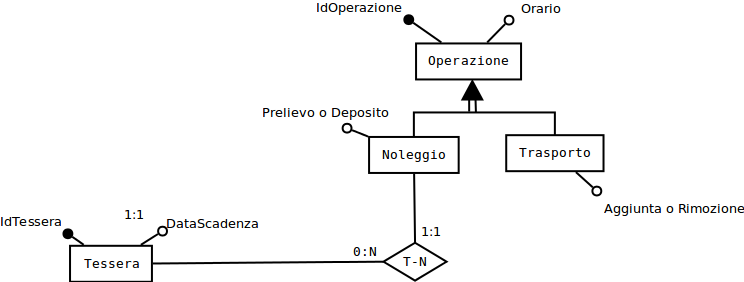
\includegraphics[width=1\textwidth]{Logico01}
\caption{Modifica a Operazione}
\end{figure}
\newpage
\subsection{Schema logico finale}
Lo schema Logico risultate.
\begin{figure}[H]
 \centering
  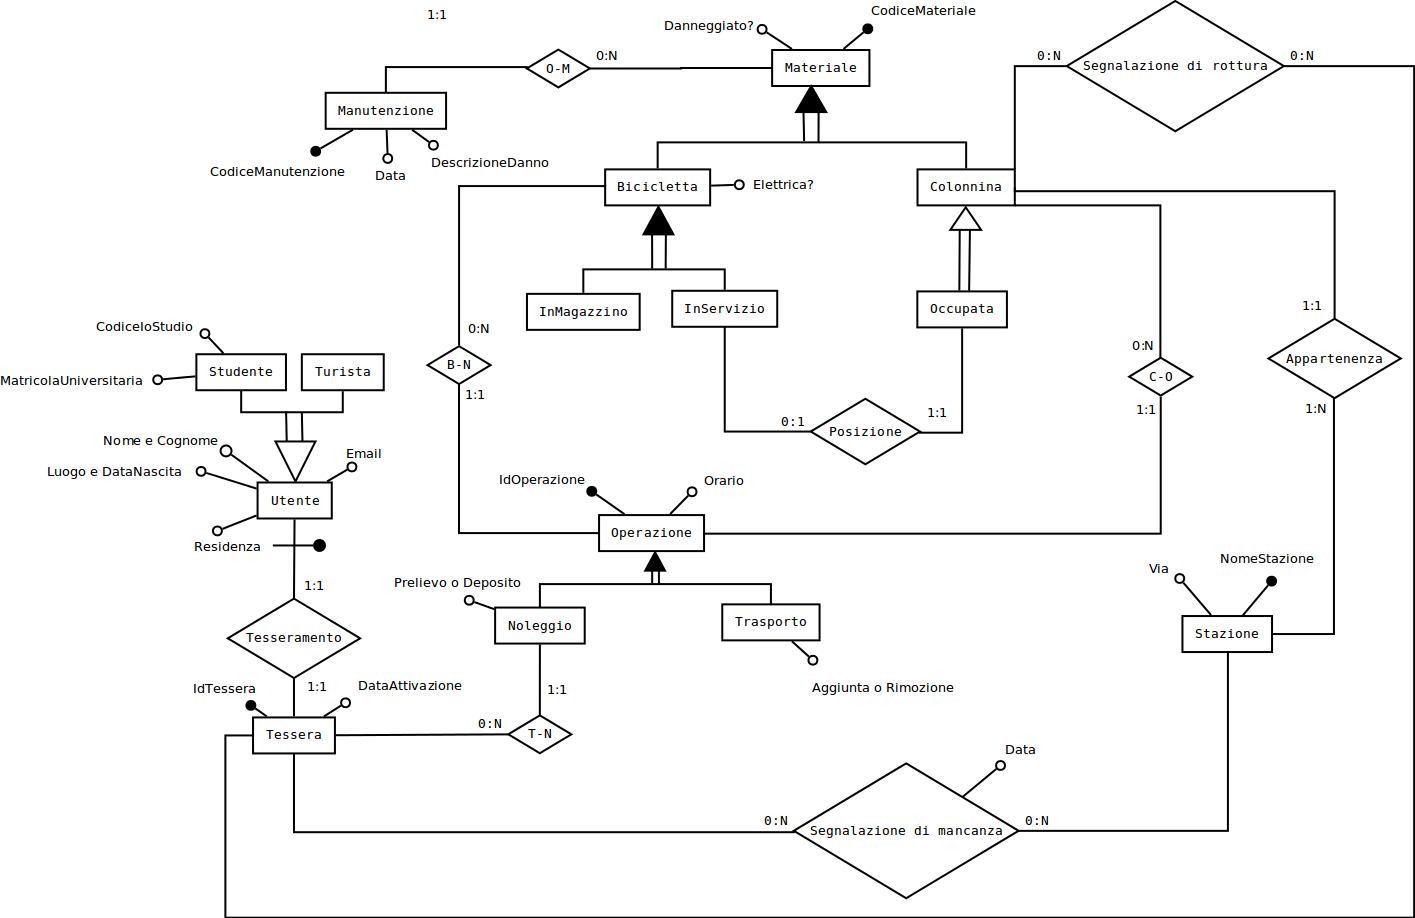
\includegraphics[width=1.35\textwidth,angle=90]{LogicoFinale}
\caption{Modello Logico Finale}
\end{figure}
\newpage
\section{Implementazione dello schema logico}
\subsection{Conversione iniziale}
Implementando lo schema logico con mysql si modificano varie parti di esso.\newline
Una prima conversione risultante dall'eliminazione delle relazioni tra le entità, rappresentate con l'aggiunta delle chiavi esterne: Segnalazione di Mancanza e Segnalazione di Rottura diventano entità (in quanto relazioni N:N).\newline
Inoltre si compiono varie scelte su come rappresentare i sottoinsiemi delle entità:
\begin{itemize}
 \item per Operazione, Bicicletta, Utente, e Colonnina si sceglie di compattare il tutto nell'entità e di aggiungere degli attributi di controllo, su cui sarà però necessario dei trigger o controlli aggiuntivi
 \item per Materiale si sceglie invece di creare 2 entità aggiuntive, in quanto sarebbe sennò stato necessario una serie di controlli complicati e un rallentamento non indifferente del sistema.
\end{itemize}
\begin{figure}[H]
 \centering
  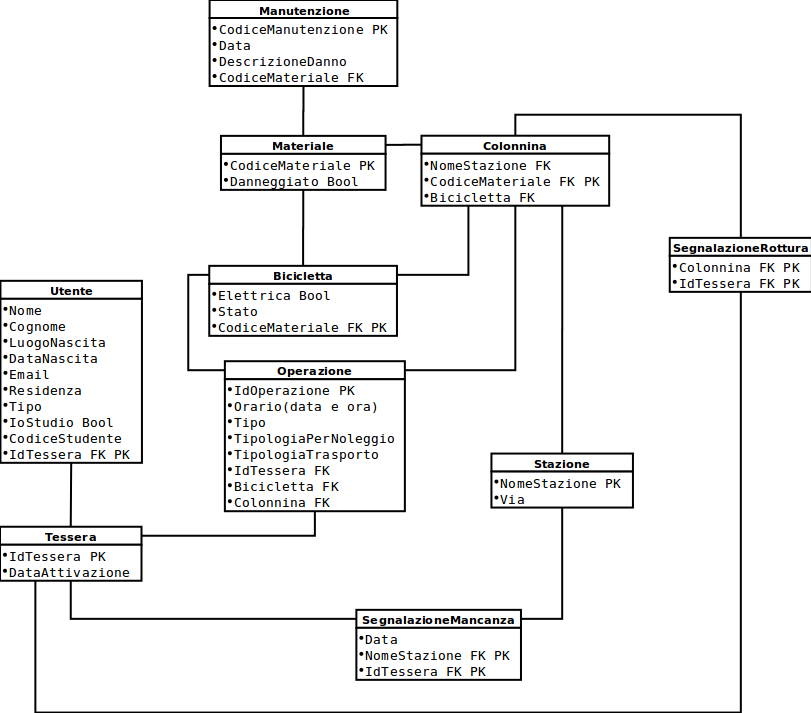
\includegraphics[width=0.8\textwidth]{SQL}
\caption{Trasformazione in SQL}
\end{figure}
\subsection{Codice sql}
Si decide di implementare i controlli sono sulle operazioni che verranno effettivamente eseguite (non ci si preoccupa ad esempio della modifica della chiave primaria di materiale, perchè non viene permesso di farlo).\newline
\subsubsection{Tessera}
\begin{lstlisting}[ language=SQL, showspaces=false, basicstyle=\ttfamily, numbers=none, numberstyle=\tiny, commentstyle=\color{gray} ]
CREATE TABLE Tessera(
IdTessera INTEGER UNSIGNED AUTO_INCREMENT,
DataAttivazione DATE NOT NULL,
PRIMARY KEY(IdTessera)
)ENGINE=INNODB;
\end{lstlisting}
\subsubsection{Utente}
\begin{lstlisting}[ language=SQL, showspaces=false, basicstyle=\ttfamily, numbers=none, numberstyle=\tiny, commentstyle=\color{gray} ]
CREATE TABLE Utente(
Nome VARCHAR(20) NOT NULL,
Cognome VARCHAR(20) NOT NULL,
DataNascita DATE NOT NULL,
LuogoNascita VARCHAR(20) NOT NULL,
Residenza VARCHAR(20) NOT NULL,
Indirizzo VARCHAR(30) NOT NULL,
Email VARCHAR(30) NOT NULL,
Tipo ENUM('Utente','Turista','Studente') DEFAULT 'Utente'
 NOT NULL,
CodiceStudente CHAR(10),
IoStudio BOOLEAN,
IdTessera INTEGER UNSIGNED,
PRIMARY KEY(IdTessera),
UNIQUE(Email),
FOREIGN KEY (IdTessera) REFERENCES Tessera(IdTessera)
 ON DELETE CASCADE
)ENGINE=INNODB;
\end{lstlisting}
\subsubsection{Materiale}
\begin{lstlisting}[ language=SQL, showspaces=false, basicstyle=\ttfamily, numbers=none, numberstyle=\tiny, commentstyle=\color{gray} ]
CREATE TABLE Materiale(
CodiceMateriale INTEGER UNSIGNED AUTO_INCREMENT,
Danneggiato BOOLEAN DEFAULT 0 NOT NULL,
PRIMARY KEY(CodiceMateriale)
)ENGINE=INNODB;
\end{lstlisting}
\subsubsection{Bicicletta}
\begin{lstlisting}[ language=SQL, showspaces=false, basicstyle=\ttfamily, numbers=none, numberstyle=\tiny, commentstyle=\color{gray} ]
CREATE TABLE Bicicletta(
CodiceMateriale INTEGER UNSIGNED,
Elettrica BOOLEAN DEFAULT 0 NOT NULL,
Stato ENUM('InServizio','InMagazzino') DEFAULT 'InMagazzino'
 NOT NULL,
PRIMARY KEY(CodiceMateriale),
FOREIGN KEY (CodiceMateriale) REFERENCES Materiale(CodiceMateriale)
 ON DELETE CASCADE
)ENGINE=INNODB;
\end{lstlisting}
\subsubsection{Stazione}
\begin{lstlisting}[ language=SQL, showspaces=false, basicstyle=\ttfamily, numbers=none, numberstyle=\tiny, commentstyle=\color{gray} ]
CREATE TABLE Stazione(
NomeStazione VARCHAR(20),
Via VARCHAR(30) NOT NULL,
PRIMARY KEY(NomeStazione)
)ENGINE=INNODB;
\end{lstlisting}
\subsubsection{Colonnina}
\begin{lstlisting}[ language=SQL, showspaces=false, basicstyle=\ttfamily, numbers=none, numberstyle=\tiny, commentstyle=\color{gray} ]
CREATE TABLE Colonnina(
CodiceMateriale INTEGER UNSIGNED,
Bicicletta INTEGER UNSIGNED DEFAULT NULL,
NomeStazione VARCHAR(20) NOT NULL,
PRIMARY KEY(CodiceMateriale),
UNIQUE(Bicicletta),
FOREIGN KEY (CodiceMateriale) REFERENCES Materiale(CodiceMateriale)
 ON DELETE CASCADE,
FOREIGN KEY (Bicicletta) REFERENCES Bicicletta(CodiceMateriale)
 ON DELETE SET NULL,
FOREIGN KEY (NomeStazione) REFERENCES Stazione(NomeStazione)
 ON DELETE CASCADE ON UPDATE CASCADE
)ENGINE=INNODB;
\end{lstlisting}
\subsubsection{Operazione}
\begin{lstlisting}[ language=SQL, showspaces=false, basicstyle=\ttfamily, numbers=none, numberstyle=\tiny, commentstyle=\color{gray} ]
CREATE TABLE Operazione(
IdOperazione INTEGER UNSIGNED AUTO_INCREMENT,
Orario DATETIME NOT NULL,
Colonnina INTEGER UNSIGNED NOT NULL,
Bicicletta INTEGER UNSIGNED NOT NULL,
Motivazione ENUM('Prelievo','Deposito','Aggiunta','Rimozione')
 NOT NULL,
IdTessera INTEGER UNSIGNED,
PRIMARY KEY(IdOperazione),
FOREIGN KEY (Colonnina) REFERENCES Colonnina(CodiceMateriale)
 ON DELETE CASCADE,
FOREIGN KEY (Bicicletta) REFERENCES Bicicletta(CodiceMateriale)
 ON DELETE CASCADE,
FOREIGN KEY (IdTessera) REFERENCES Tessera(IdTessera)
 ON DELETE CASCADE
)ENGINE=INNODB;
\end{lstlisting}
Ora però si osserva come Tipo,TipologiaPerNoleggio e TipologiaTrasporto siamo una brutta rappresentazione di come un'operazione possa essere di tipo 'Prelievo', 'Deposito', 'Aggiunta' o 'Rimozione', quindi si sostituiscono con un unico Attributo.
\begin{lstlisting}[ language=SQL, showspaces=false, basicstyle=\ttfamily, numbers=none, numberstyle=\tiny, commentstyle=\color{gray} ]
CREATE TABLE Operazione(
IdOperazione INTEGER UNSIGNED AUTO_INCREMENT,
Orario DATETIME NOT NULL,
Colonnina INTEGER UNSIGNED NOT NULL,
Bicicletta INTEGER UNSIGNED NOT NULL,
Motivazione ENUM('Prelievo','Deposito','Aggiunta','Rimozione')
 NOT NULL,
IdTessera INTEGER UNSIGNED,
PRIMARY KEY(IdOperazione),
UNIQUE(Orario,Colonnina),
FOREIGN KEY (Colonnina) REFERENCES Colonnina(CodiceMateriale)
 ON DELETE CASCADE,
FOREIGN KEY (Bicicletta) REFERENCES Bicicletta(CodiceMateriale)
 ON DELETE CASCADE,
FOREIGN KEY (IdTessera) REFERENCES Tessera(IdTessera)
 ON DELETE CASCADE
)ENGINE=INNODB;
\end{lstlisting}
\subsubsection{Manutenzione}
\begin{lstlisting}[ language=SQL, showspaces=false, basicstyle=\ttfamily, numbers=none, numberstyle=\tiny, commentstyle=\color{gray} ]
CREATE TABLE Manutenzione(
NumeroManutenzione INTEGER UNSIGNED AUTO_INCREMENT,
DataManutenzione DATE NOT NULL,
DescrizioneDanno VARCHAR(100),
CodiceMateriale INTEGER UNSIGNED NOT NULL,
PRIMARY KEY(NumeroManutenzione),
FOREIGN KEY (CodiceMateriale) REFERENCES Materiale(CodiceMateriale)
 ON DELETE CASCADE
)ENGINE=INNODB;
\end{lstlisting}
\subsubsection{Segnalazione Rottura}
\begin{lstlisting}[ language=SQL, showspaces=false, basicstyle=\ttfamily, numbers=none, numberstyle=\tiny, commentstyle=\color{gray} ]
CREATE TABLE SegnalazioneRottura(
Colonnina INTEGER UNSIGNED,
IdTessera INTEGER UNSIGNED,
PRIMARY KEY(IdTessera,Colonnina),
FOREIGN KEY (Colonnina) REFERENCES Colonnina(CodiceMateriale)
 ON DELETE CASCADE,
FOREIGN KEY (IdTessera) REFERENCES Tessera(IdTessera)
 ON DELETE CASCADE
)ENGINE=INNODB;
\end{lstlisting}
\subsubsection{Segnalazione Mancanza}
\begin{lstlisting}[ language=SQL, showspaces=false, basicstyle=\ttfamily, numbers=none, numberstyle=\tiny, commentstyle=\color{gray} ]
CREATE TABLE SegnalazioneMancanza(
NomeStazione VARCHAR(20),
IdTessera INTEGER UNSIGNED,
DataSegnalazione DATE NOT NULL,
PRIMARY KEY(IdTessera,NomeStazione),
FOREIGN KEY (NomeStazione) REFERENCES Stazione(NomeStazione)
 ON DELETE CASCADE,
FOREIGN KEY (IdTessera) REFERENCES Tessera(IdTessera)
 ON DELETE CASCADE
)ENGINE=INNODB;
\end{lstlisting}
\section{Query, procedure, trigger e funzioni}
\subsection{Query}
\subsection{Trigger}
\subsubsection{\texttt{insert\_utente}}
Se un nuovo Utente ha come Tipo 'Studente' allora CodiceStudente e IoStudio non possono essere nulli, se non é 'Studente' allora devono essere nulli.
\begin{lstlisting}[ language=SQL, showspaces=false, basicstyle=\ttfamily, numbers=none, numberstyle=\tiny, commentstyle=\color{gray} ]
CREATE TRIGGER insert_utente
BEFORE INSERT ON Utente
FOR EACH ROW BEGIN
DECLARE idT INTEGER UNSIGNED;
DECLARE dat DATE;
SELECT CURDATE() INTO dat;
INSERT INTO Tessera(DataAttivazione) VALUES (dat);
SELECT Tessera.IdTessera INTO idT FROM Tessera
ORDER BY Tessera.IdTessera DESC LIMIT 1;
SET NEW.IdTessera = idT;
IF NEW.Tipo = 'Utente' OR NEW.Tipo = 'Turista'
THEN SET NEW.CodiceStudente = NULL;
SET NEW.IoStudio = NULL;
ElSE IF NEW.CodiceStudente IS NULL OR
NEW.IoStudio IS NULL
THEN SET NEW.IdTessera = NULL;
END IF; END IF;
END;
\end{lstlisting}
\subsubsection{\texttt{delete\_tessera}}
Per eliminare una tessera deve non essere in corso nessun noleggio su quella tessera.
\begin{lstlisting}[ language=SQL, showspaces=false, basicstyle=\ttfamily, numbers=none, numberstyle=\tiny, commentstyle=\color{gray} ]
CREATE TRIGGER delete_tessera
AFTER DELETE ON Tessera
FOR EACH ROW BEGIN
DECLARE mot ENUM('Prelievo','Deposito','Aggiunta','Rimozione');
SELECT Operazione.Motivazione INTO mot
FROM Operazione
WHERE Operazione.IdTessera = OLD.IdTessera
ORDER BY Operazione.Orario DESC LIMIT 1;
IF mot = 'Prelievo' THEN
INSERT INTO Tessera(IdTessera) VALUES (NULL);
END IF;
END;
\end{lstlisting}
\subsubsection{\texttt{insert\_bicicletta}}
All'inserimento di una bicicletta viene creato un materiale e usato quel materiale come chiave per la bicicletta.
\begin{lstlisting}[ language=SQL, showspaces=false, basicstyle=\ttfamily, numbers=none, numberstyle=\tiny, commentstyle=\color{gray} ]
CREATE TRIGGER insert_bicicletta
BEFORE INSERT ON Bicicletta
FOR EACH ROW BEGIN
DECLARE num INTEGER UNSIGNED;
INSERT INTO Materiale(Danneggiato) VALUES (0);
SELECT Materiale.CodiceMateriale INTO num FROM Materiale
ORDER BY Materiale.CodiceMateriale DESC LIMIT 1;
SET NEW.CodiceMateriale = num;
END;
\end{lstlisting}
\subsubsection{\texttt{delete\_bicicletta}}
L'eliminazione di una bicicletta è possibile sono se non è utilizzata in un noleggio.
\begin{lstlisting}[ language=SQL, showspaces=false, basicstyle=\ttfamily, numbers=none, numberstyle=\tiny, commentstyle=\color{gray} ]
CREATE TRIGGER delete_bicicletta
AFTER DELETE ON Bicicletta
FOR EACH ROW BEGIN
DECLARE mot ENUM('Prelievo','Deposito','Aggiunta','Rimozione');
SELECT Operazione.Motivazione INTO mot FROM Operazione WHERE
Operazione.Bicicletta = OLD.CodiceMateriale
ORDER BY Operazione.Orario DESC LIMIT 1;
IF mot = 'Prelievo' THEN
INSERT INTO Materiale(CodiceMateriale) VALUES (NULL);
END IF;
END;
\end{lstlisting}
\subsubsection{\texttt{insert\_colonnina}}
Come per Bicicletta viene creato anche qui un nuovo materiale corrispondente alla bicicletta.
\begin{lstlisting}[ language=SQL, showspaces=false, basicstyle=\ttfamily, numbers=none, numberstyle=\tiny, commentstyle=\color{gray} ]
CREATE TRIGGER insert_colonnina
BEFORE INSERT ON Colonnina
FOR EACH ROW BEGIN
DECLARE num INTEGER UNSIGNED;
INSERT INTO Materiale(Danneggiato) VALUES (0);
SELECT Materiale.CodiceMateriale INTO num FROM Materiale
ORDER BY Materiale.CodiceMateriale DESC LIMIT 1;
SET NEW.CodiceMateriale = num;
END;
\end{lstlisting}
\subsubsection{\texttt{delete\_colonnina}}
Se si elimina una colonnina la bici (se presente) viene riportata in magazzino.
\begin{lstlisting}[ language=SQL, showspaces=false, basicstyle=\ttfamily, numbers=none, numberstyle=\tiny, commentstyle=\color{gray} ]
CREATE TRIGGER delete_colonnina
AFTER DELETE ON Colonnina
FOR EACH ROW BEGIN
IF OLD.Bicicletta IS NOT NULL THEN UPDATE Bicicletta
SET Stato = 'InMagazzino'
WHERE Bicicletta.CodiceMateriale = OLD.Bicicletta;
END IF;
END;
\end{lstlisting}
\subsubsection{\texttt{insert\_operazione}}
Su operazione si fanno molti controlli in base al tipo di essa (la motivazione):
\begin{itemize}
 \item per un prelievo o un deposito si verifica che IdTessera non sia nullo, poi si controlla che quell'operazione non sia successiva ad un'operazione analoga, essendo possibile solo un noleggio alla volta, infine si modifica lo stato della colonnina in base all'operazione avvenuta
 \item per un'aggiunta o una rimozione si mette a NULL la tessera e si modifica lo stato di servizio della bicicletta tra InServizio o InMagazzino e si modifica di conseguenza la presenza della bicicletta in colonnina
\end{itemize}
In ogni caso il trigger si preoccupa di inserire la data e come ultima operazione elimina le segnalazioni si mancanza della stazione in cui la colonnina fa parte.
\begin{lstlisting}[ language=SQL, showspaces=false, basicstyle=\ttfamily, numbers=none, numberstyle=\tiny, commentstyle=\color{gray} ]
CREATE TRIGGER insert_operazione
BEFORE INSERT ON Operazione
FOR EACH ROW BEGIN
DECLARE nol BOOLEAN;
DECLARE mot ENUM('Prelievo','Deposito','Aggiunta','Rimozione');
DECLARE dat DATETIME;
SET nol = FALSE;
SELECT NOW() INTO dat;
SET NEW.Orario = dat;
IF NEW.Motivazione = 'Prelievo' OR NEW.Motivazione = 'Deposito' THEN
IF NEW.IdTessera IS NULL THEN SET NEW.IdOperazione = NULL;
END IF;
SELECT Operazione.Motivazione INTO mot FROM Operazione WHERE
Operazione.IdTessera = NEW.IdTessera AND Operazione.Motivazione = 'Prelievo'
AND Operazione.IdOperazione <> NEW.IdOperazione ORDER BY Operazione.Orario
 DESC LIMIT 1;
IF mot = 'Prelievo' THEN SET nol = TRUE; END IF;
IF NEW.Motivazione = 'Prelievo' THEN IF nol = TRUE THEN
SET NEW.IdOperazione = NULL;
ElSE UPDATE Colonnina SET Colonnina.Bicicletta = NULL WHERE
Colonnina.CodiceMateriale = NEW.Colonnina;
END IF; END IF;
IF NEW.Motivazione = 'Deposito' THEN IF nol = FALSE THEN
SET NEW.IdOperazione = NULL;
ELSE UPDATE Colonnina SET Colonnina.Bicicletta = NEW.Bicicletta WHERE
Colonnina.CodiceMateriale = NEW.Colonnina;
END IF; END IF;
ELSE
IF NEW.Motivazione = 'Aggiunta' THEN
IF NEW.IdTessera IS NOT NULL THEN SET NEW.IdTessera = NULL;
END IF;
UPDATE Bicicletta SET Bicicletta.Stato = 'InServizio' WHERE
Bicicletta.CodiceMateriale = NEW.Bicicletta;
UPDATE Colonnina SET Colonnina.Bicicletta = NEW.Bicicletta WHERE
Colonnina.CodiceMateriale = NEW.Colonnina;
END IF;
IF NEW.Motivazione = 'Rimozione' THEN
IF NEW.IdTessera IS NOT NULL THEN SET NEW.IdTessera = NULL;
END IF;
UPDATE Bicicletta SET Bicicletta.Stato = 'InMagazzino' WHERE
Bicicletta.CodiceMateriale = NEW.Bicicletta;
UPDATE Colonnina SET Colonnina.Bicicletta = NULL WHERE
Colonnina.CodiceMateriale = NEW.Colonnina;
END IF; END IF;
DELETE FROM SegnalazioneMancanza WHERE
SegnalazioneMancanza.NomeStazione = (
 SELECT Colonnina.NomeStazione FROM Colonnina WHERE
 NEW.Colonnina = Colonnina.CodiceMateriale LIMIT 1);
END;
\end{lstlisting}
\subsubsection{\texttt{insert\_manutenzione}}
All'inserimento di una manutenzione vengono cancellate tutte le segnalazioni relative alla colonnina e viene aggiornato il materiale rimuovendo il booleano che rappresenta lo stato danneggiato. Viene anche inserita la data esatta.
\begin{lstlisting}[ language=SQL, showspaces=false, basicstyle=\ttfamily, numbers=none, numberstyle=\tiny, commentstyle=\color{gray} ]
CREATE TRIGGER insert_manutenzione
BEFORE INSERT ON Manutenzione
FOR EACH ROW BEGIN
DECLARE dat DATE;
DECLARE bic INTEGER UNSIGNED;
SELECT CURDATE() INTO dat;
SET NEW.DataManutenzione = dat;
DELETE FROM SegnalazioneRottura WHERE
NEW.CodiceMateriale = SegnalazioneRottura.Colonnina;
UPDATE Materiale SET Materiale.Danneggiato = FALSE WHERE
NEW.CodiceMateriale = Materiale.CodiceMateriale;
SELECT Colonnina.Bicicletta INTO bic FROM Colonnina WHERE
NEW.CodiceMateriale = Colonnina.CodiceMateriale;
IF bic IS NOT NULL THEN
UPDATE Materiale SET Materiale.Danneggiato = FALSE WHERE
bic = Materiale.CodiceMateriale;
END IF;
END;
\end{lstlisting}
\subsubsection{\texttt{insert\_segnalazione\_rottura}}
La segnalazione di rottura aggiorna lo stato della colonnina e della bici se presente, segnalandole come materiale danneggiato.
\begin{lstlisting}[ language=SQL, showspaces=false, basicstyle=\ttfamily, numbers=none, numberstyle=\tiny, commentstyle=\color{gray} ]
CREATE TRIGGER insert_segnalazione_rottura
BEFORE INSERT ON SegnalazioneRottura
FOR EACH ROW BEGIN
UPDATE Materiale SET Materiale.Danneggiato = TRUE WHERE
NEW.Colonnina = Materiale.CodiceMateriale;
UPDATE Materiale JOIN Colonnina ON
Materiale.CodiceMateriale = Colonnina.Bicicletta AND
NEW.Colonnina = Colonnina.CodiceMateriale
SET Materiale.Danneggiato = TRUE WHERE
NEW.Colonnina = Colonnina.CodiceMateriale;
END;
\end{lstlisting}
\subsubsection{\texttt{insert\_segnalazione\_mancanza}}
La segnalazione di mancanza inserisce la data corretta, poi controlla se si è veramente con una stazione completamente piena o completamente vuota; solo in questi casi si può fare una segnalazione.
\begin{lstlisting}[ language=SQL, showspaces=false, basicstyle=\ttfamily, numbers=none, numberstyle=\tiny, commentstyle=\color{gray} ]
CREATE TRIGGER insert_segnalazione_mancanza
BEFORE INSERT ON SegnalazioneMancanza
FOR EACH ROW BEGIN
DECLARE dat DATE;
SELECT CURDATE() INTO dat;
SET NEW.DataSegnalazione = dat;
END;
\end{lstlisting}
\newpage
\section{Interfaccia web}
L'applicazione web è composta da un'area riservata all'utente e una dedicata all'amministrazione e trasporto/manutenzione.
Per comodità visto la natura accademica del progetto e per facilitare la correzione, sono state differenziate le aree già nella pagina iniziale dove è possibile fare il login inserendo un IdTessera valido (int unsigned incrementale) per accedere alle funzionalità per l'utente mentre cliccando gli appositi link si accederà alle funzioni riservate ai tecnici per le riparazioni, trasportatori per trasportare le biciclette e amministratori per poter aggiungere e rimuovere utenti, colonnine, stazioni e bici: 
\begin{figure}[H]
	\centering
	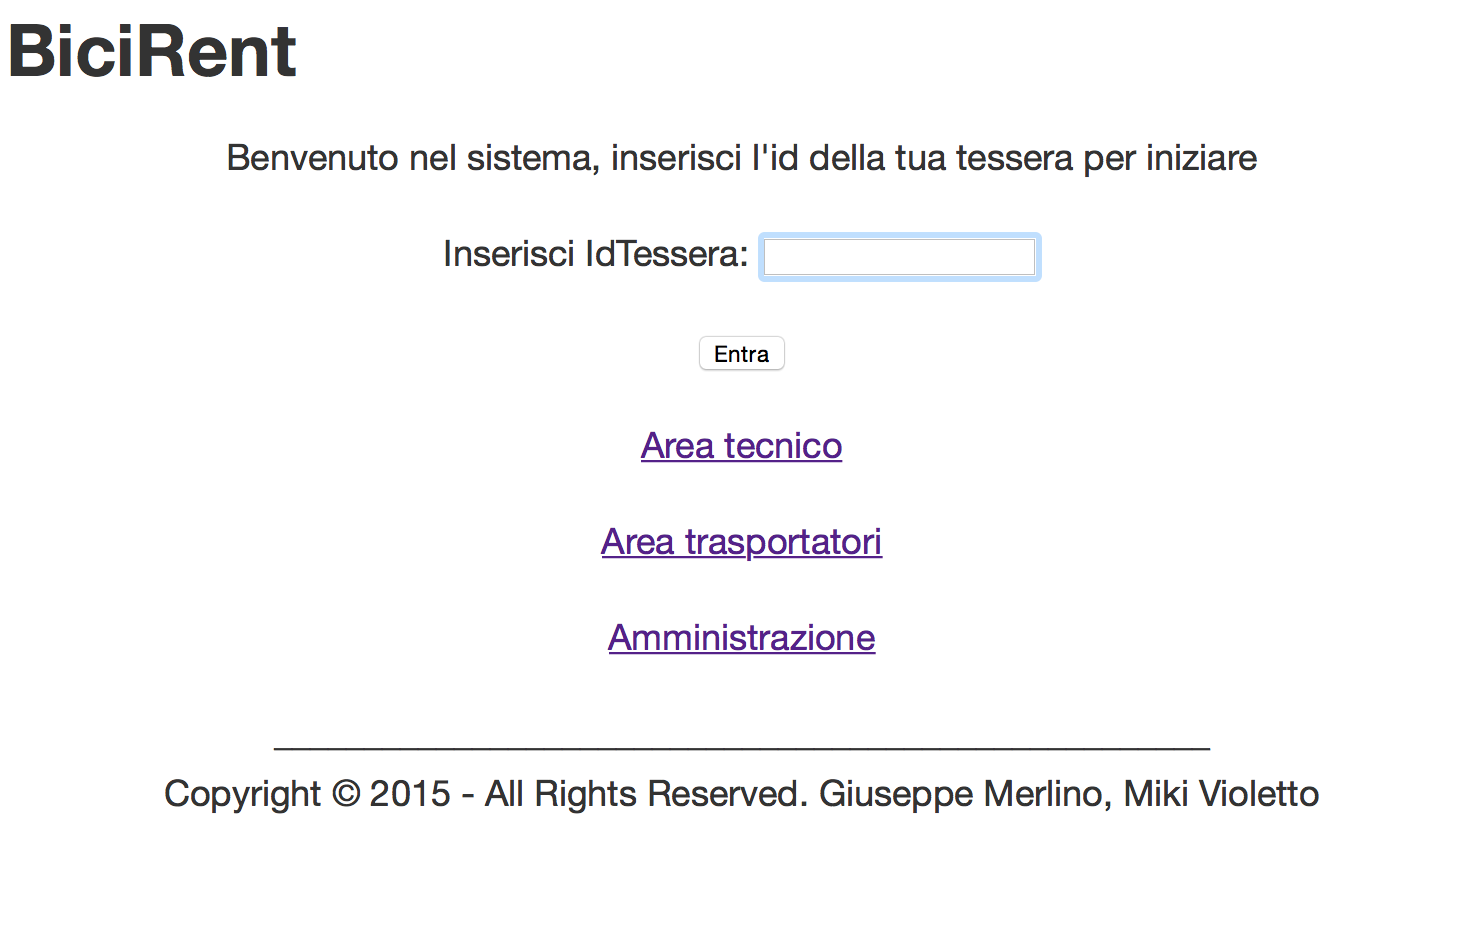
\includegraphics[width=0.8\textwidth]{Screenshot01}
	\caption{Rappresentazione index.php}
\end{figure}
\subsection{Area utente}
Una volta effettuato il login verrà creata una sessione dove vengono salvate alcune informazioni utili come la tessera e se si ha un noleggio attualmente in corso o meno in modo che la pagina possa presentare l'operazione corretta da effettuare (Noleggio o Deposito). Nella figura 21 si nota che viene presentata un elemento select dove è possibile selezionare la stazione desiderata per noleggiare o depositare la bici.
\begin{figure}[H]
	\centering
	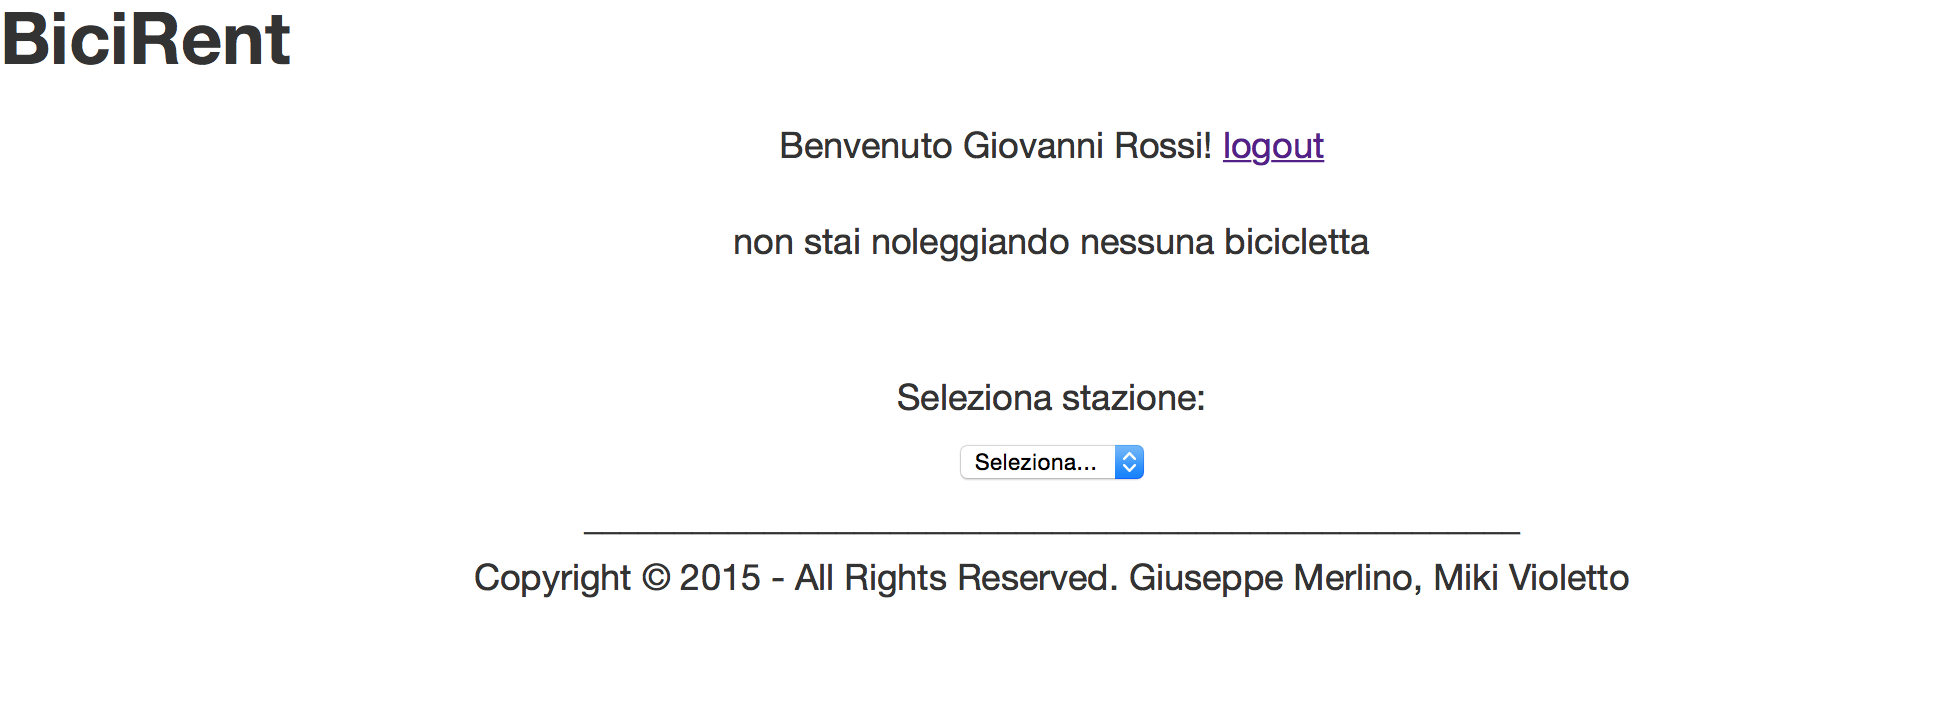
\includegraphics[width=0.8\textwidth]{Screenshot02}
	\caption{Rappresentazione iniziale utente.php}
\end{figure}
Dopo aver scelto la stazione apparirà una tabella che mostra la situazione attuale delle colonnine per poter effettuare operazioni di noleggio o segnalare la mancanza di colonnine libere quando si deposita o occupate in caso di prelievo. Inoltre è possibile segnalare ogni singola colonnina, da notare che se essa è occupata da una bicicletta anche quest'ultima verrà segnalata come guasta, inoltre è possibile effettuare una sola segnalazione per ogni colonnina da parte di ogni utente.
Le colonnine sono identificate dal loro CodiceMateriale e risultano di color rosso se occupate da una bicicletta o verdi se libere, grigie se segnalate come guaste.
I pulsanti si abilitano o disabilitano per ogni particolare caso grazie ad un'apposita funzione javascript. 
\begin{figure}[H]
	\centering
	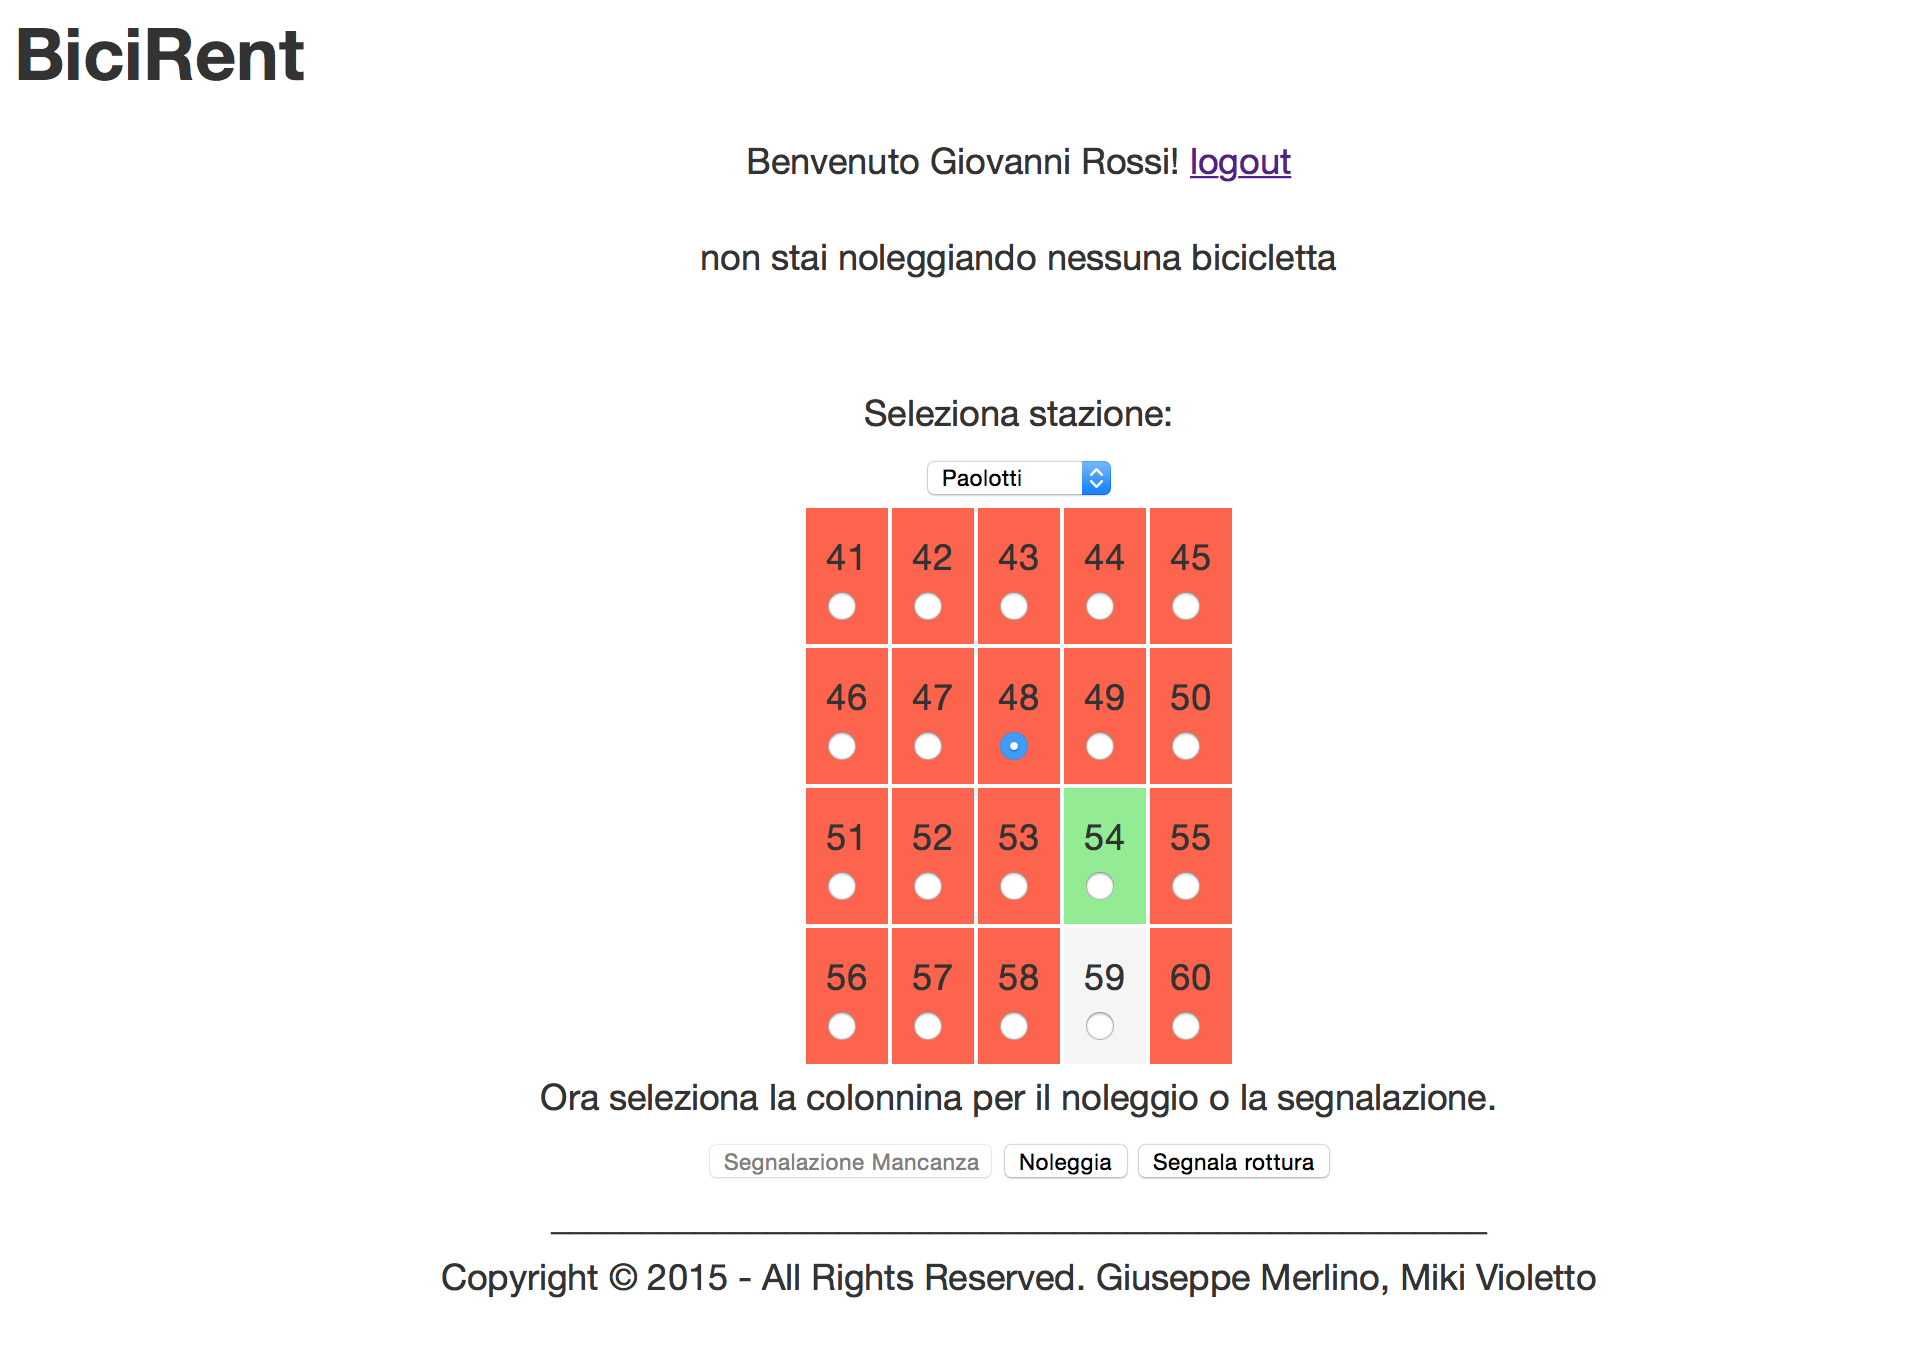
\includegraphics[width=0.8\textwidth]{Screenshot03}
	\caption{Rappresentazione espansa utente.php}
\end{figure}
Compilata correttamente la form, essa viene inviata alla pagina checkout.php che valuterà l'azione necessaria da compiere nel database.
Una volta effettuata l'operazione l'utente potrà effettuare il logout o tornare alla propria area riservata per procedere con ulteriori operazioni.
\subsection{Area tecnico}
La sezione serve per effettuare operazioni di manutenzione sulle colonnine e/o biciclette ad esse collegate. La pagina visualizza un tabella contenente le colonnine segnalate ordinate per priorità di segnalazione (in alto quelle più segnalate) modificando inoltre il colore delle righe per notare meglio le urgenze. Il manutentore cliccherà il radio button relativo alla colonnina che deve riparare e scriverà nella textarea sottostante la tabella l'operazione di manutenzione effettuata. Una volta inviata la form, la pagina verrà ricaricata e verrà visualizzato un messaggio di conferma o un errore in caso la sottomissione non vada a buon fine.
\begin{figure}[H]
	\centering
	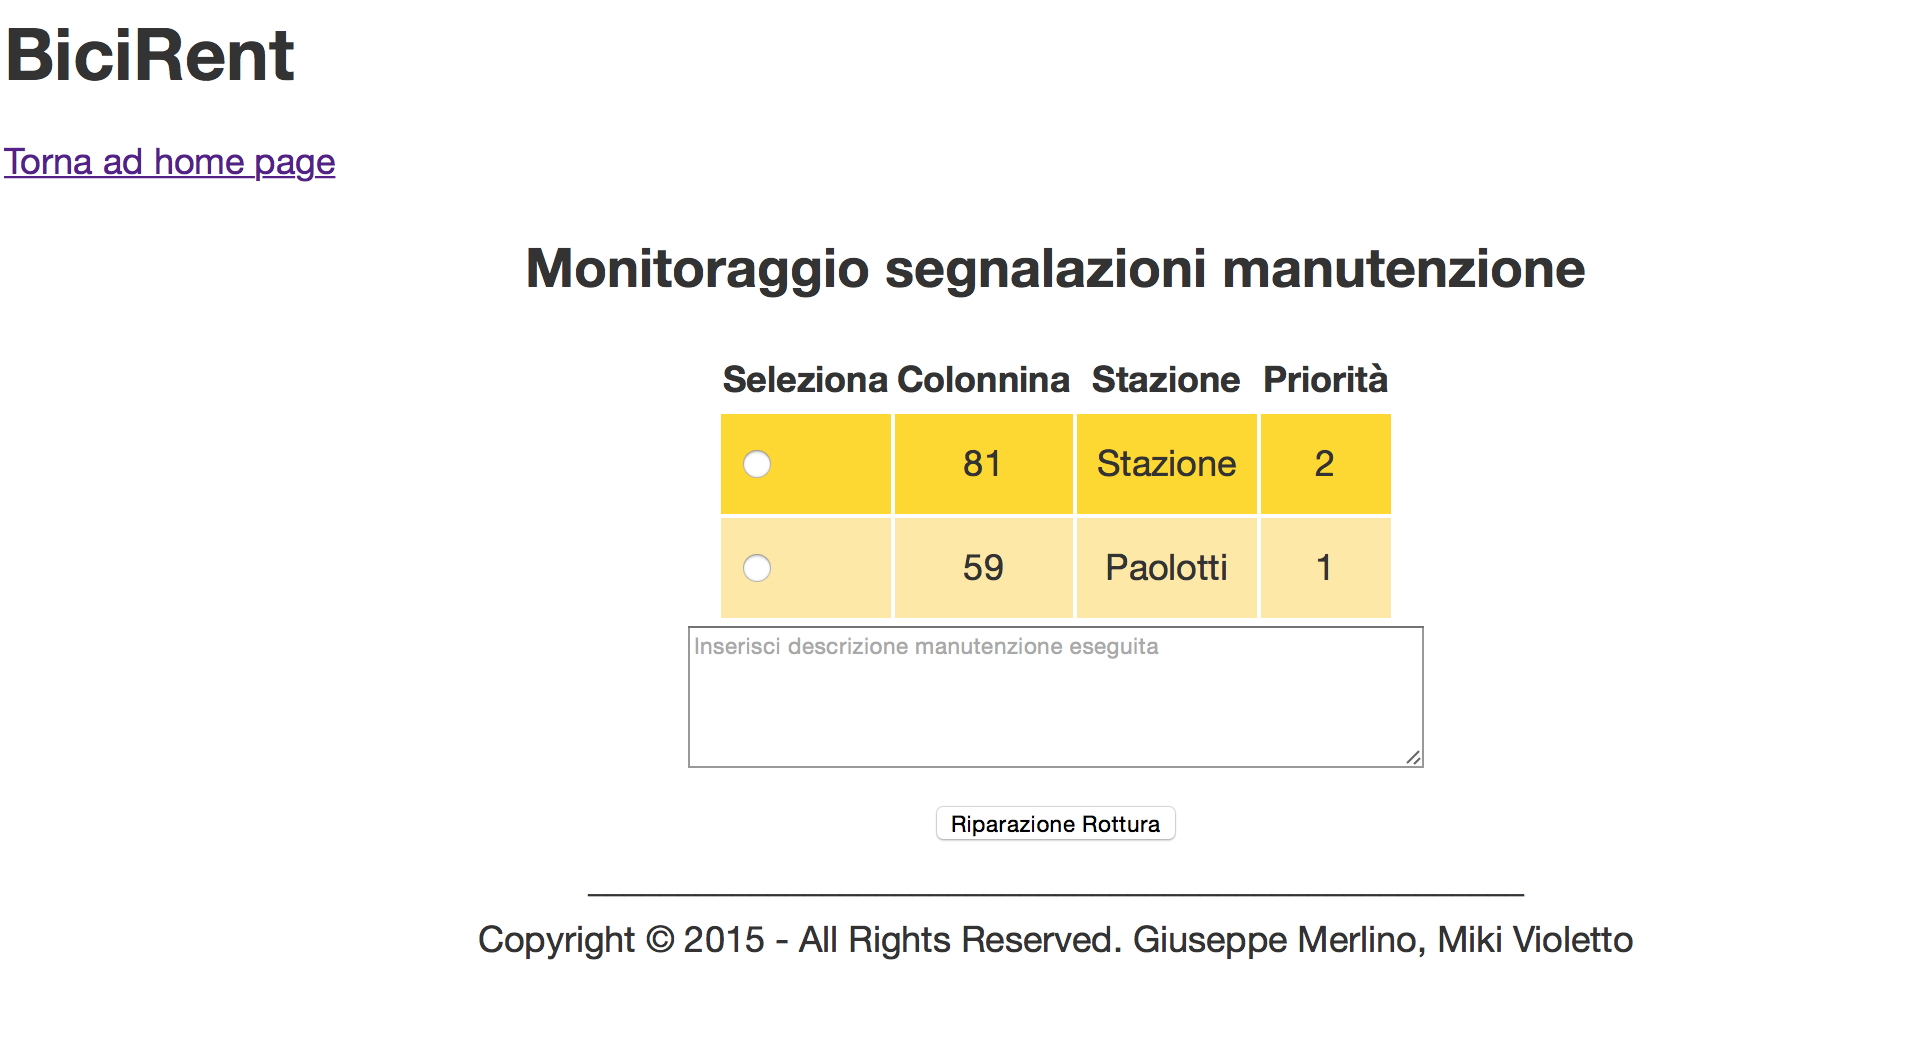
\includegraphics[width=0.8\textwidth]{Screenshot04}
	\caption{Rappresentazione tecnico.php}
\end{figure}
\subsection{Area trasportatori}
In quest'area i trasportatori potranno aggiungere o rimuovere biciclette da stazioni o dal magazzino. La pagina mostra le segnalazioni di mancanza per prelievi o depositi anche in questo caso ordinati per numero di segnalazioni effettuate. Inoltre verranno mostrate anche le stazioni dove non sono state segnalate mancanze in modo che l'impiegato possa aggiungere biciclette anche in queste stazioni. Infine si trova l'opzione del magazzino dove sarà solamente possibile trasportare delle biciclette dalle stazioni presenti. Una funzione javascript si prende carico di rimuovere il riepilogo magazzino se verrà selezionato quest'ultimo poichè non ha senso trasportare una bicicletta nel medesimo luogo, lo stesso tipo di controllo viene effettuato per il riepilogo delle stazioni in modo da disabilitare le checkbox relative alla stazione selezionata verso la quale effettuare il trasporto. Una volta scelto il luogo e le biciclette da trasportare si può cliccare sul bottone posto sotto la tabella del monitoraggio segnalazioni per effettuare l'operazione.
La pagina verrà ricaricata mostrando un esito per ogni singola bicicletta trasportata.
\begin{figure}[H]
	\centering
	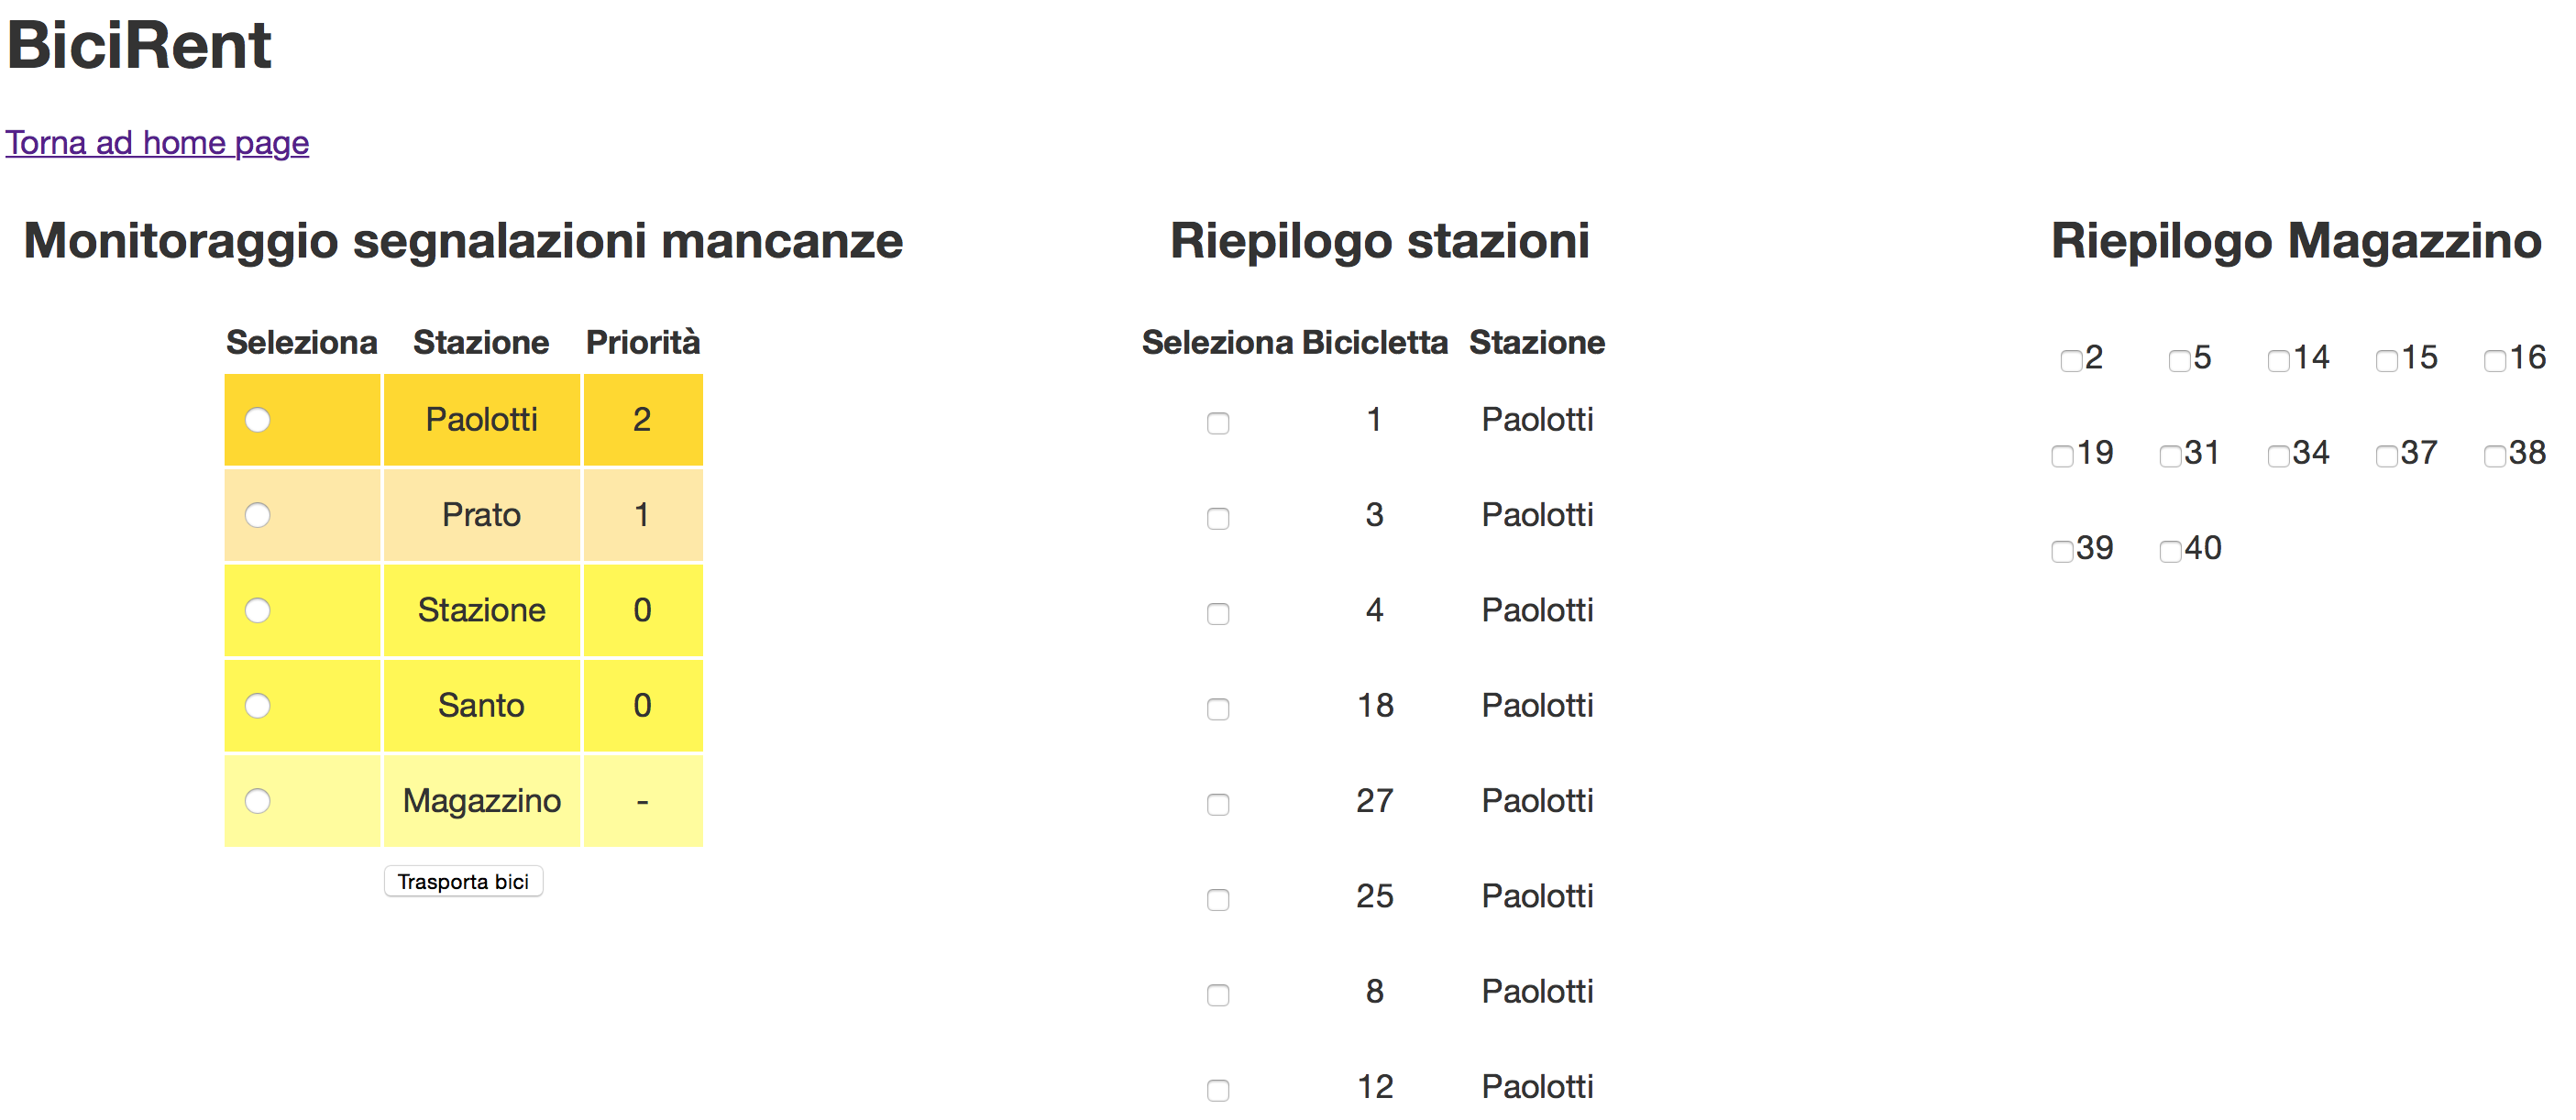
\includegraphics[width=0.8\textwidth]{Screenshot05}
	\caption{Rappresentazione trasporto.php}
\end{figure}
\subsection{Amministrazione}
A differenza delle altre pagine, quest'area sfrutta inizialmente il metodo GET per accedere alle varie sotto-categorie, da qui è possibile effettuare le tipiche operazioni di aggiunta/eliminazione.
Dopo aver selezionato l'operazione da effettuare la pagina si ricarica presentando la form corretta.
\begin{figure}[H]
	\centering
	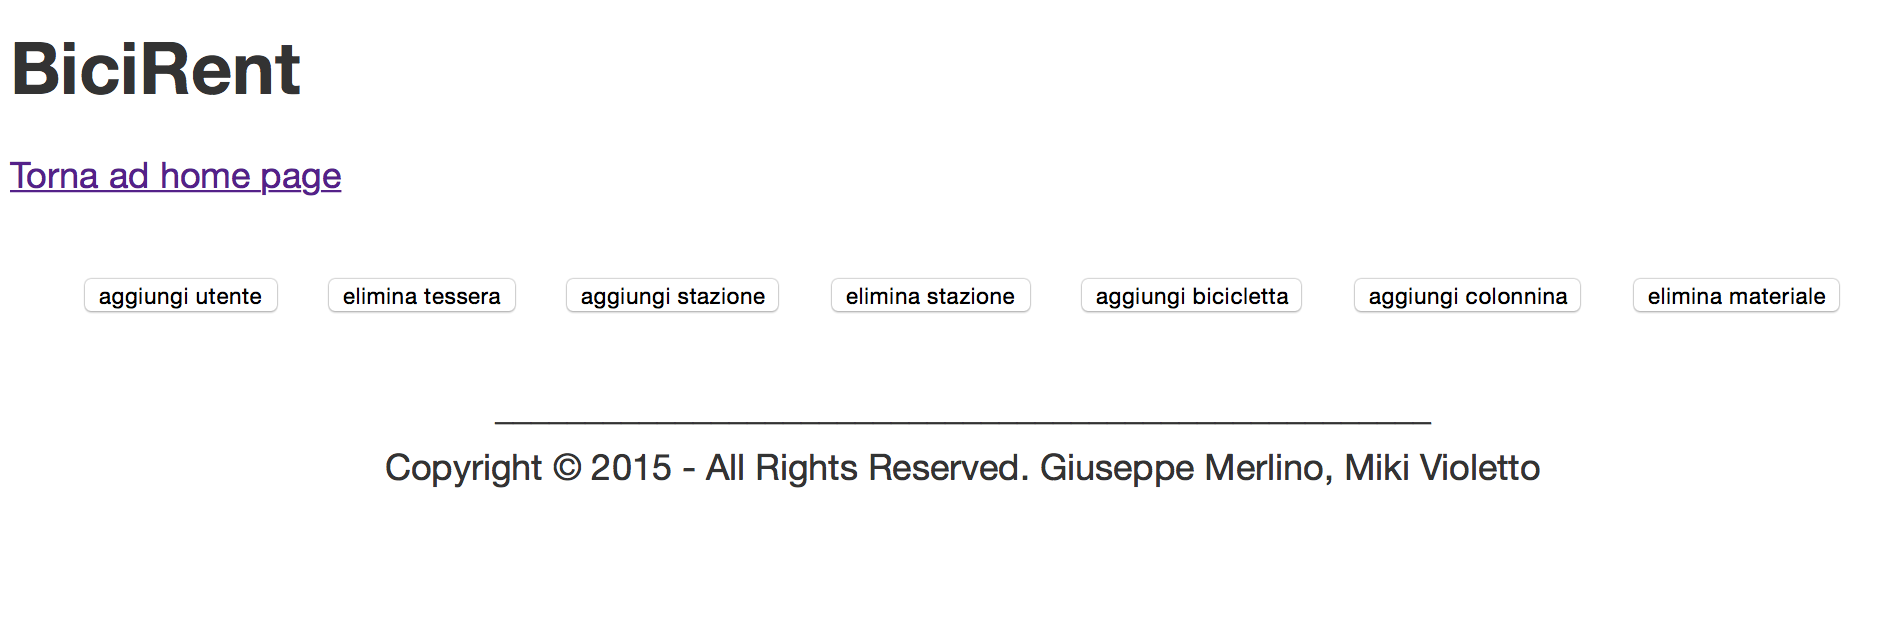
\includegraphics[width=0.8\textwidth]{Screenshot06}
	\caption{Rappresentazione admin.php}
\end{figure}
\subsubsection{Aggiungi utente}
La form permette di inserire nel database un nuovo utente e si presenta con i campi relativi alle informazioni personali, al tipo di utente che si crea e in caso esso sia uno studente, l'impiegato dovrà compilare i campi dedicati. Una volta terminato l'inserimento è possibile inviare la richiesta tramite il pulsante aggiungi utente che ricaricherà la pagina e invierà i dati con metodo POST inserendo l'esito tramite GET nell'url. Inoltre è possibile consultare la lista utenti cliccando l'apposito link.
\begin{figure}[H]
	\centering
	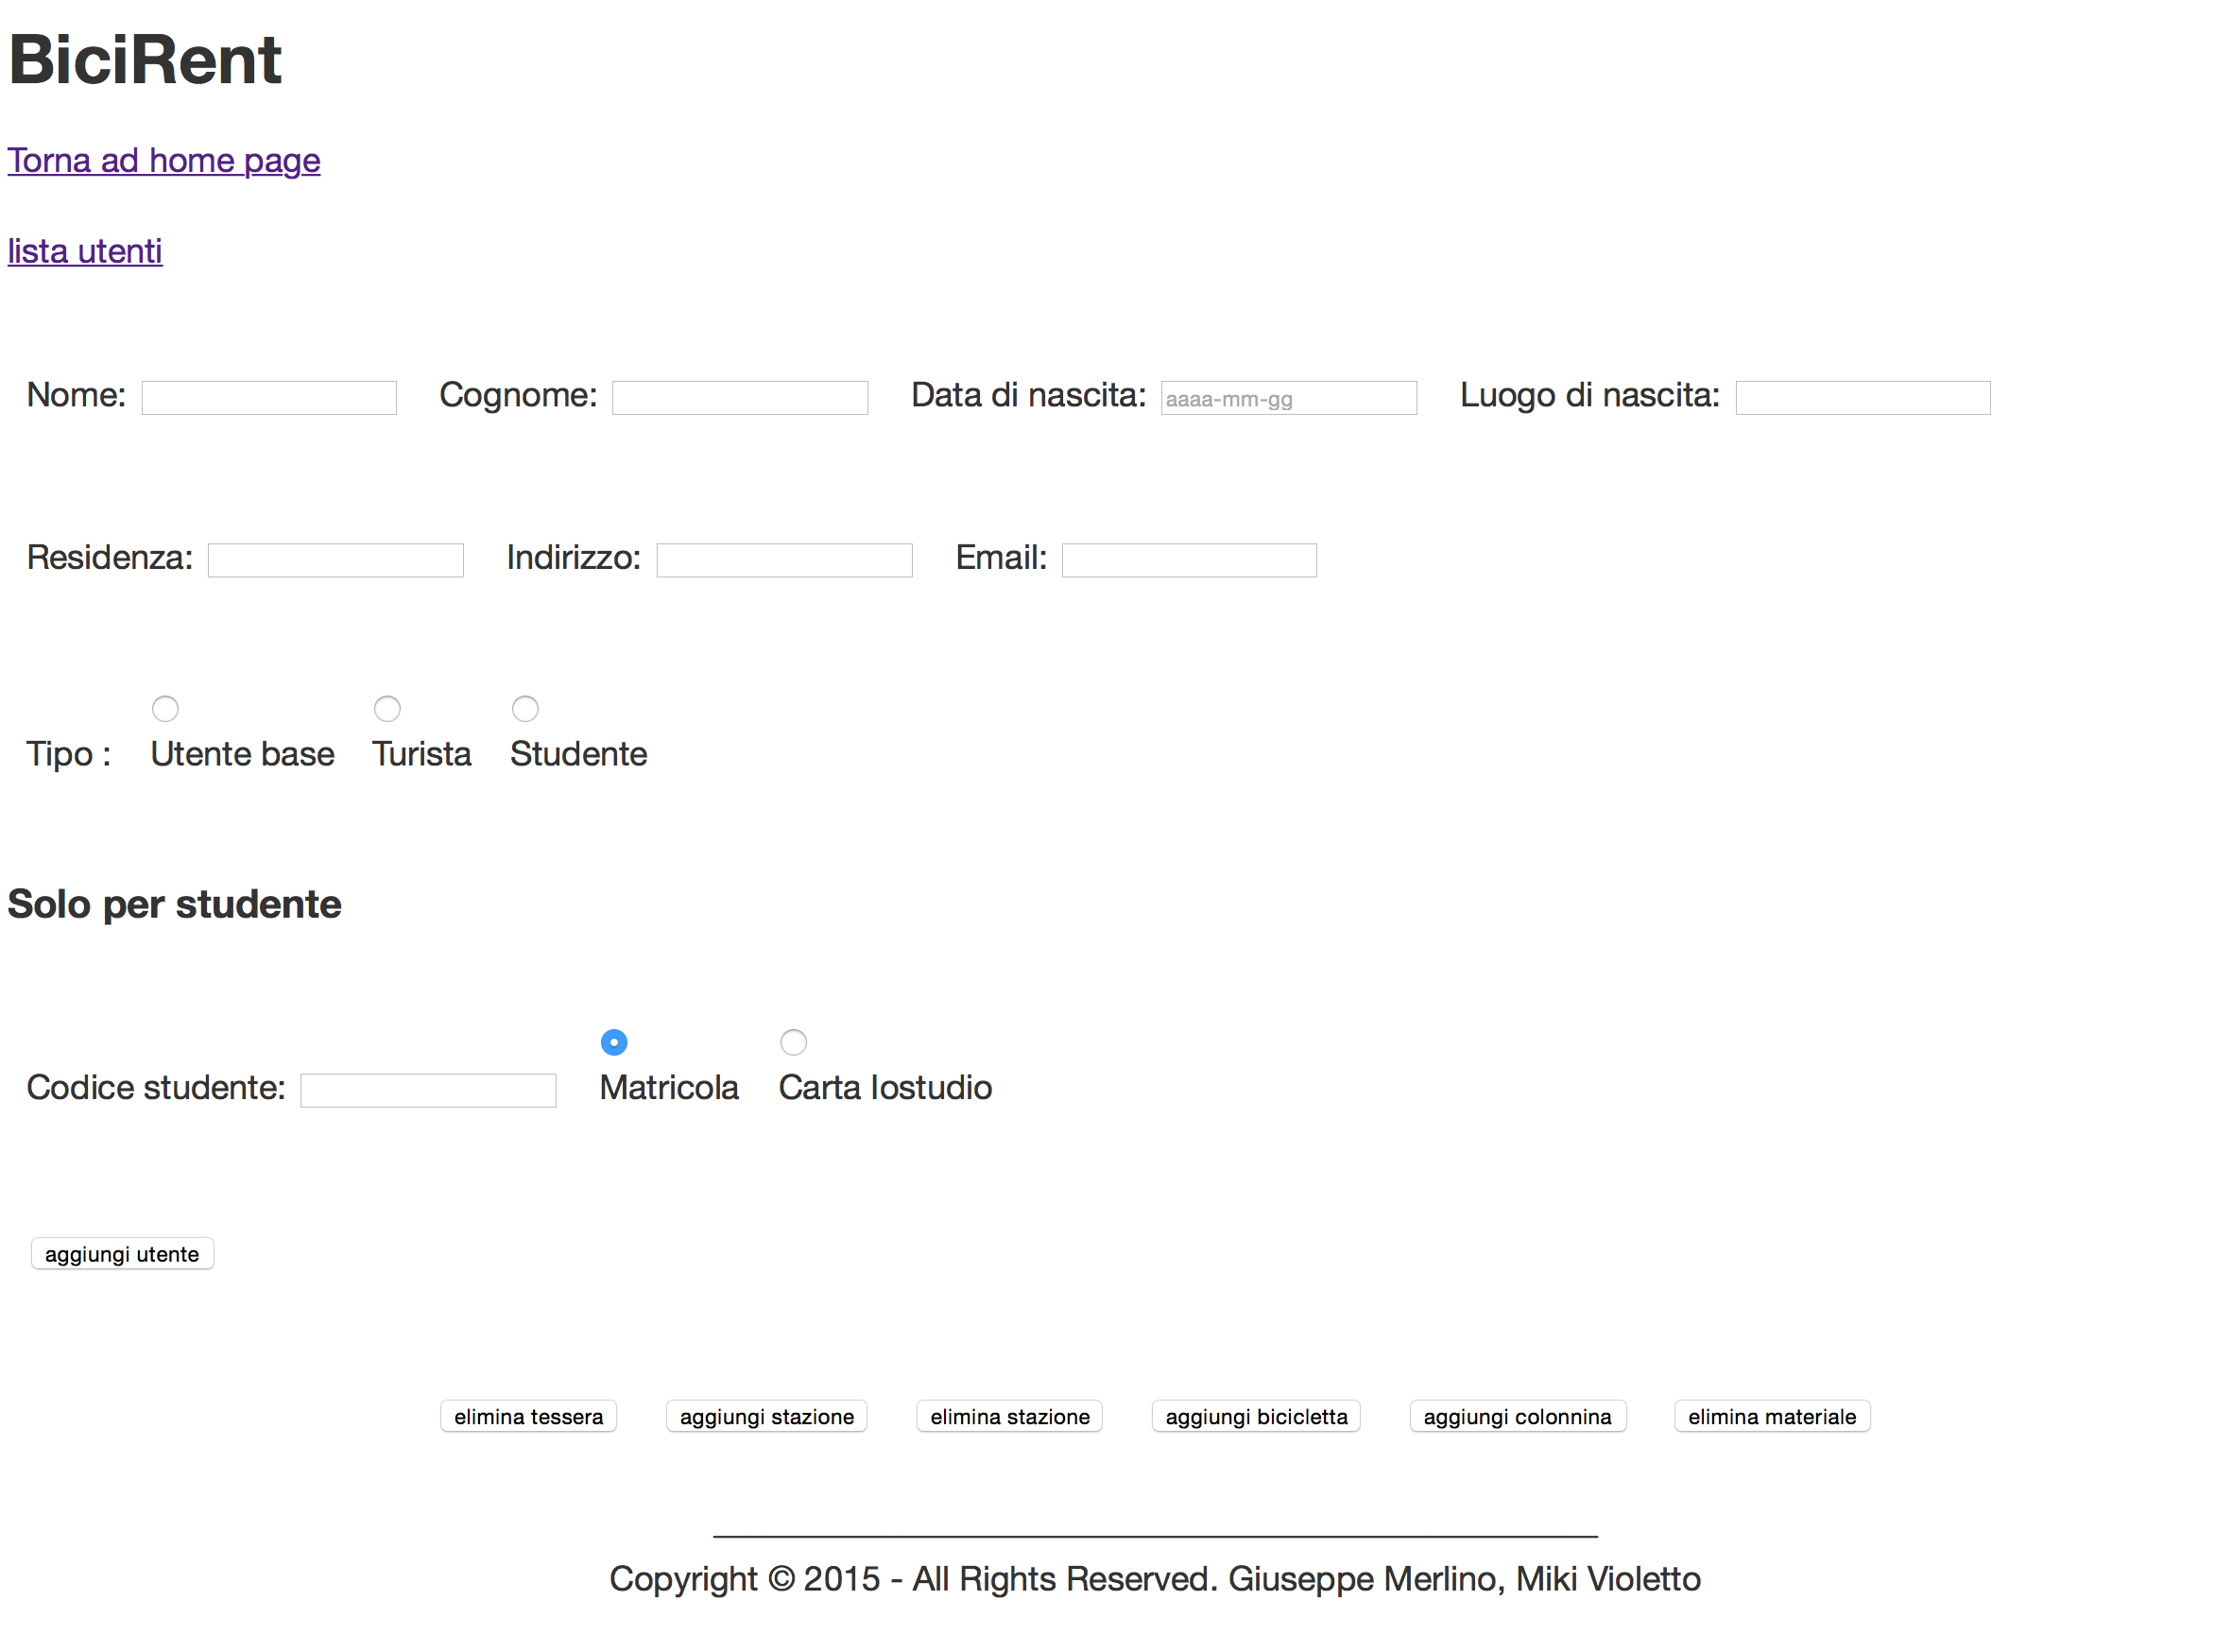
\includegraphics[width=0.8\textwidth]{Screenshot07}
	\caption{Rappresentazione admin.php?action=aggiungi+utente}
\end{figure}
\subsubsection{Aggiungi stazione}
La form permette di inserire nel database una nuova stazione e si presenta con i campi relativi al nome e alla via dove verrà aggiunta. Una volta terminato l'inserimento è possibile inviare la richiesta tramite il pulsante aggiungi stazione che ricaricherà la pagina e invierà i dati con metodo POST inserendo l'esito tramite GET nell'url. Inoltre è possibile consultare la lista stazioni cliccando l'apposito link.
\begin{figure}[H]
	\centering
	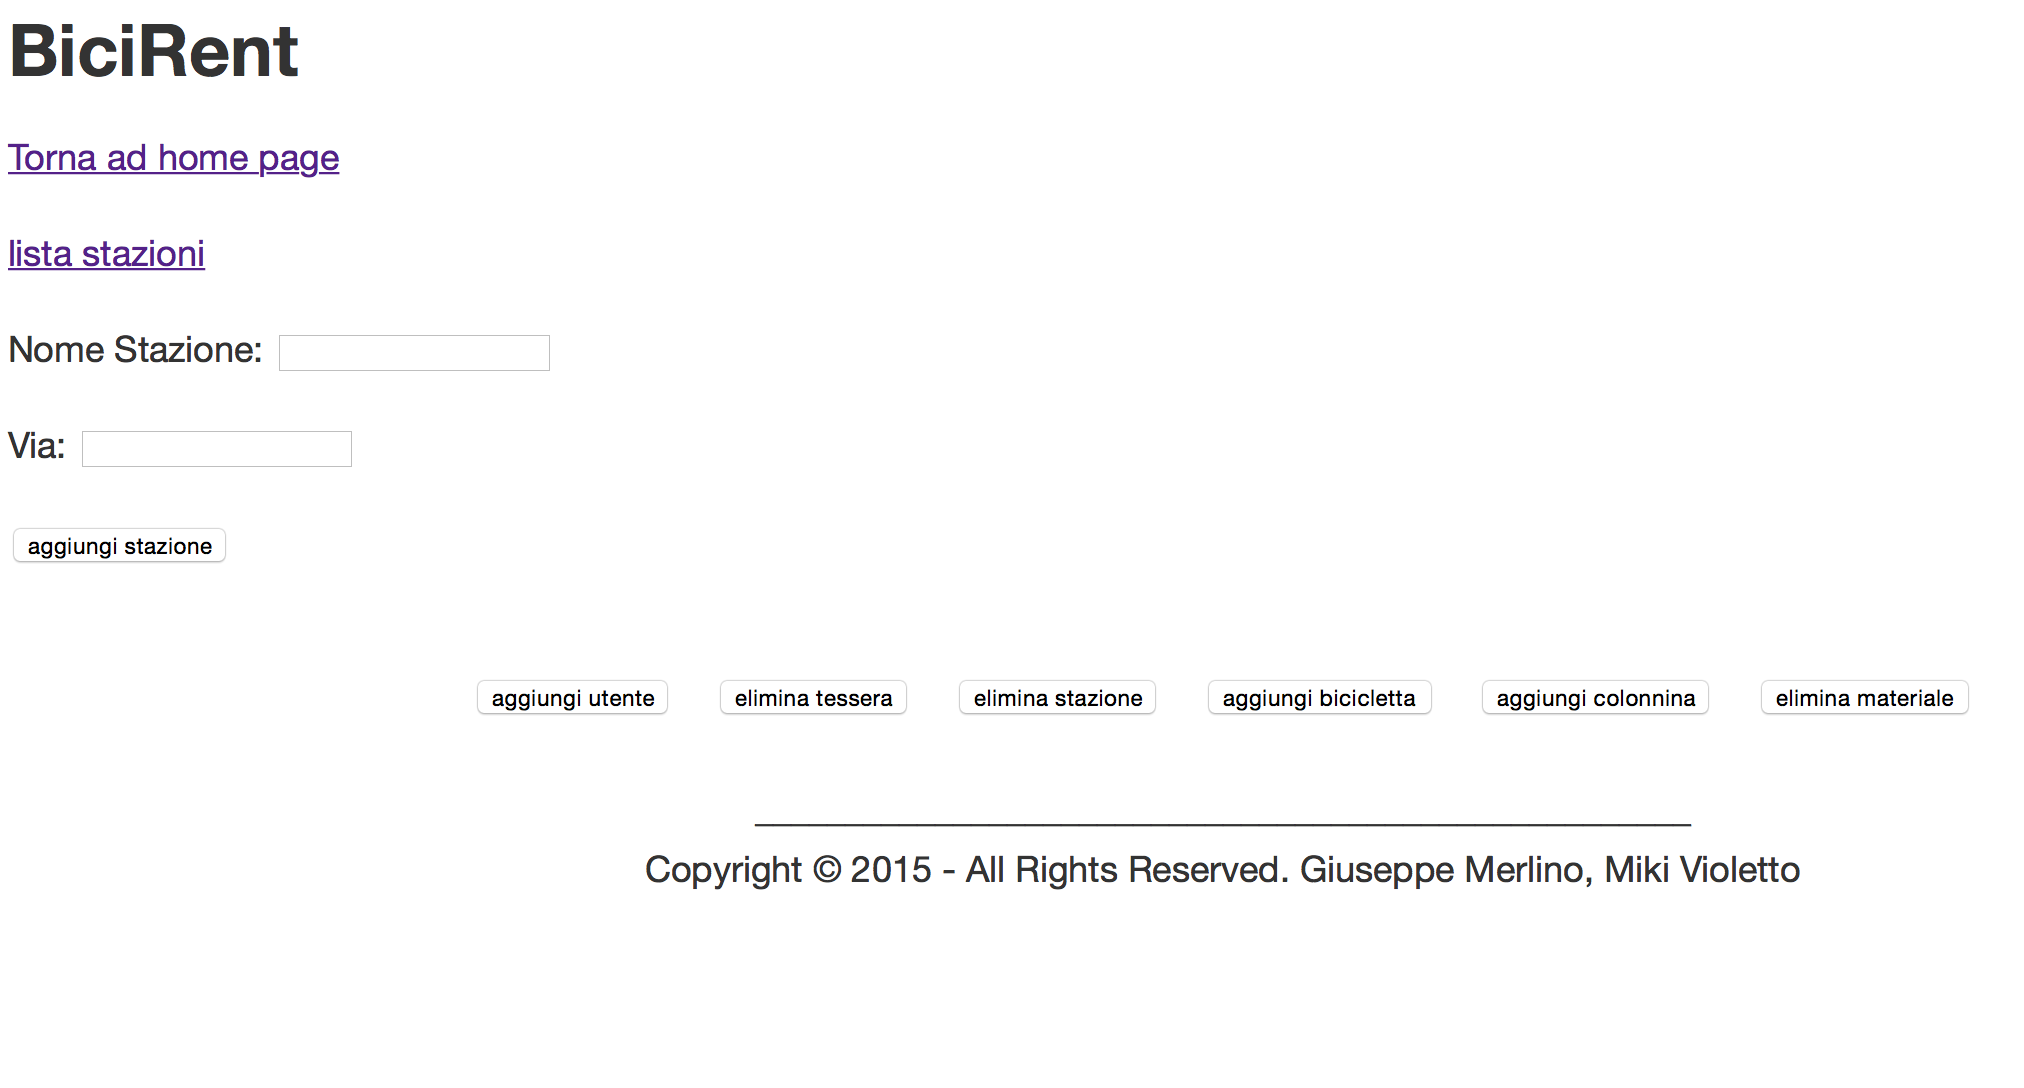
\includegraphics[width=0.8\textwidth]{Screenshot08}
	\caption{Rappresentazione admin.php?action=aggiungi+stazione}
\end{figure}
\subsubsection{Elimina tessera}
La form permette di eliminare dal database una tessera e si presenta con il campo relativo all'id da inserire per procedere alla cancellazione. Una volta terminato l'inserimento è possibile inviare la richiesta tramite il pulsante elimina tessera che ricaricherà la pagina e invierà i dati con metodo POST inserendo l'esito tramite GET nell'url. Inoltre è possibile consultare la lista tessere cliccando l'apposito link.
\begin{figure}[H]
	\centering
	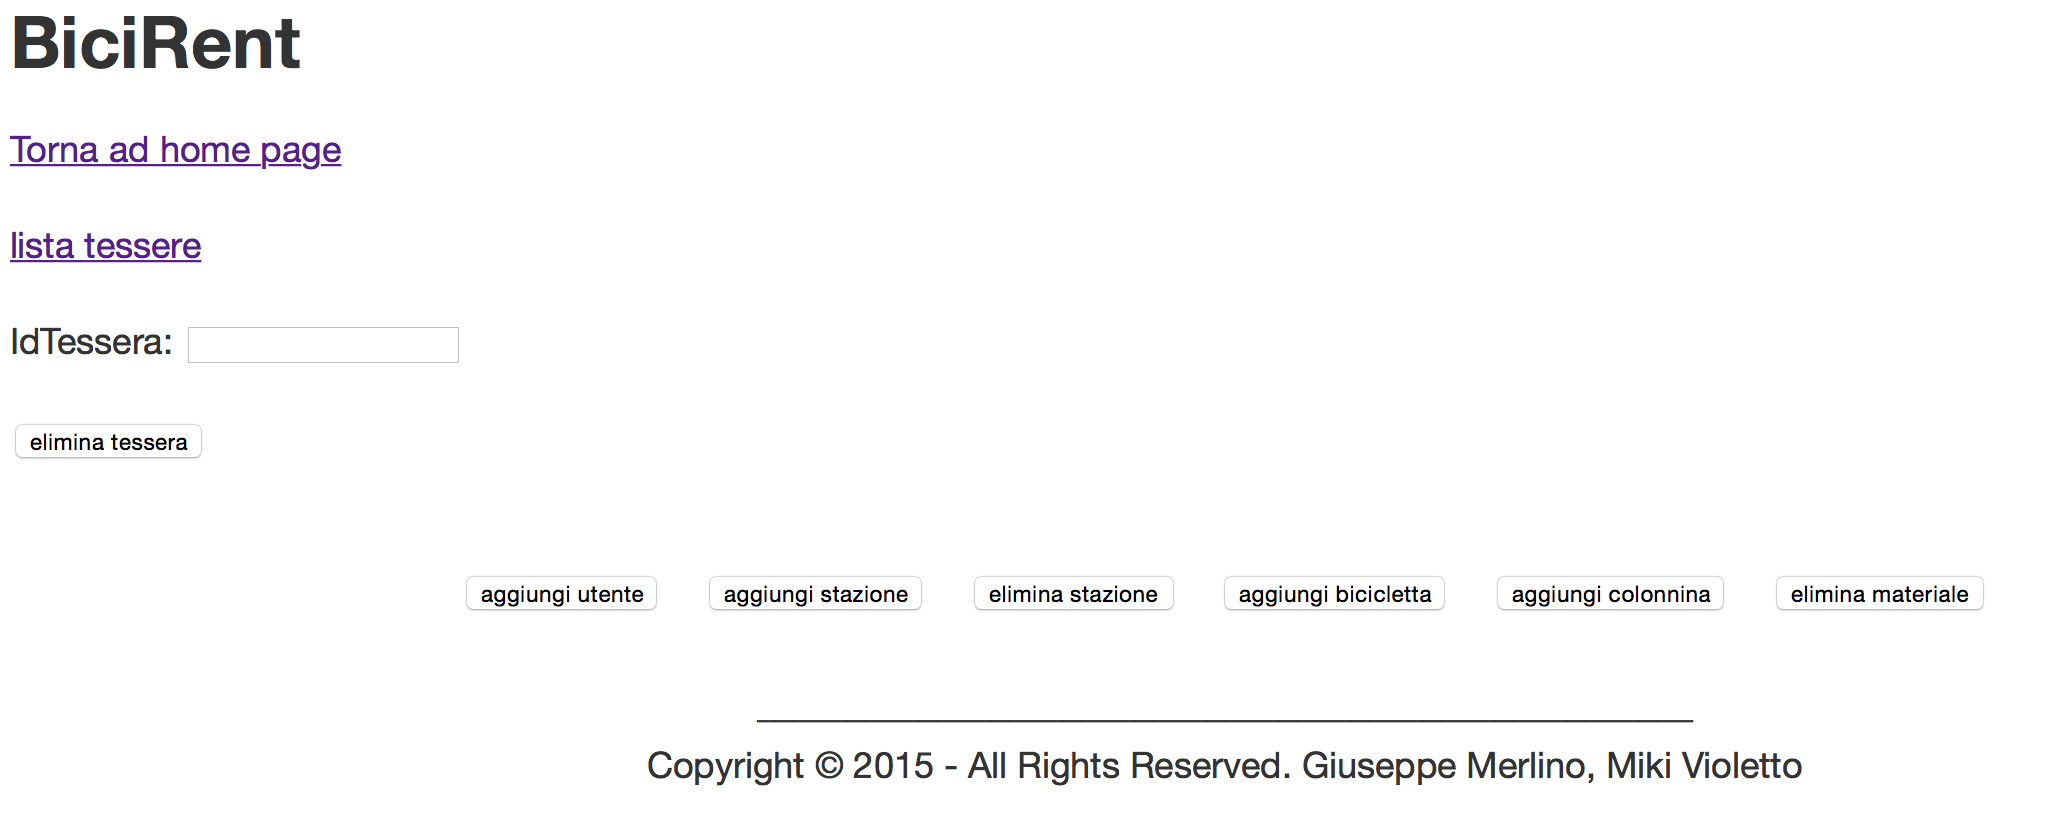
\includegraphics[width=0.8\textwidth]{Screenshot09}
	\caption{Rappresentazione admin.php?action=elimina+tessera}
\end{figure}
\subsubsection{Elimina stazione}
La form permette di eliminare dal database una stazione e si presenta con il campo relativo al nome da inserire per procedere alla cancellazione. Una volta terminato l'inserimento è possibile inviare la richiesta tramite il pulsante elimina stazione che ricaricherà la pagina e invierà i dati con metodo POST inserendo l'esito tramite GET nell'url. Inoltre è possibile consultare la lista stazioni cliccando l'apposito link.
\begin{figure}[H]
	\centering
	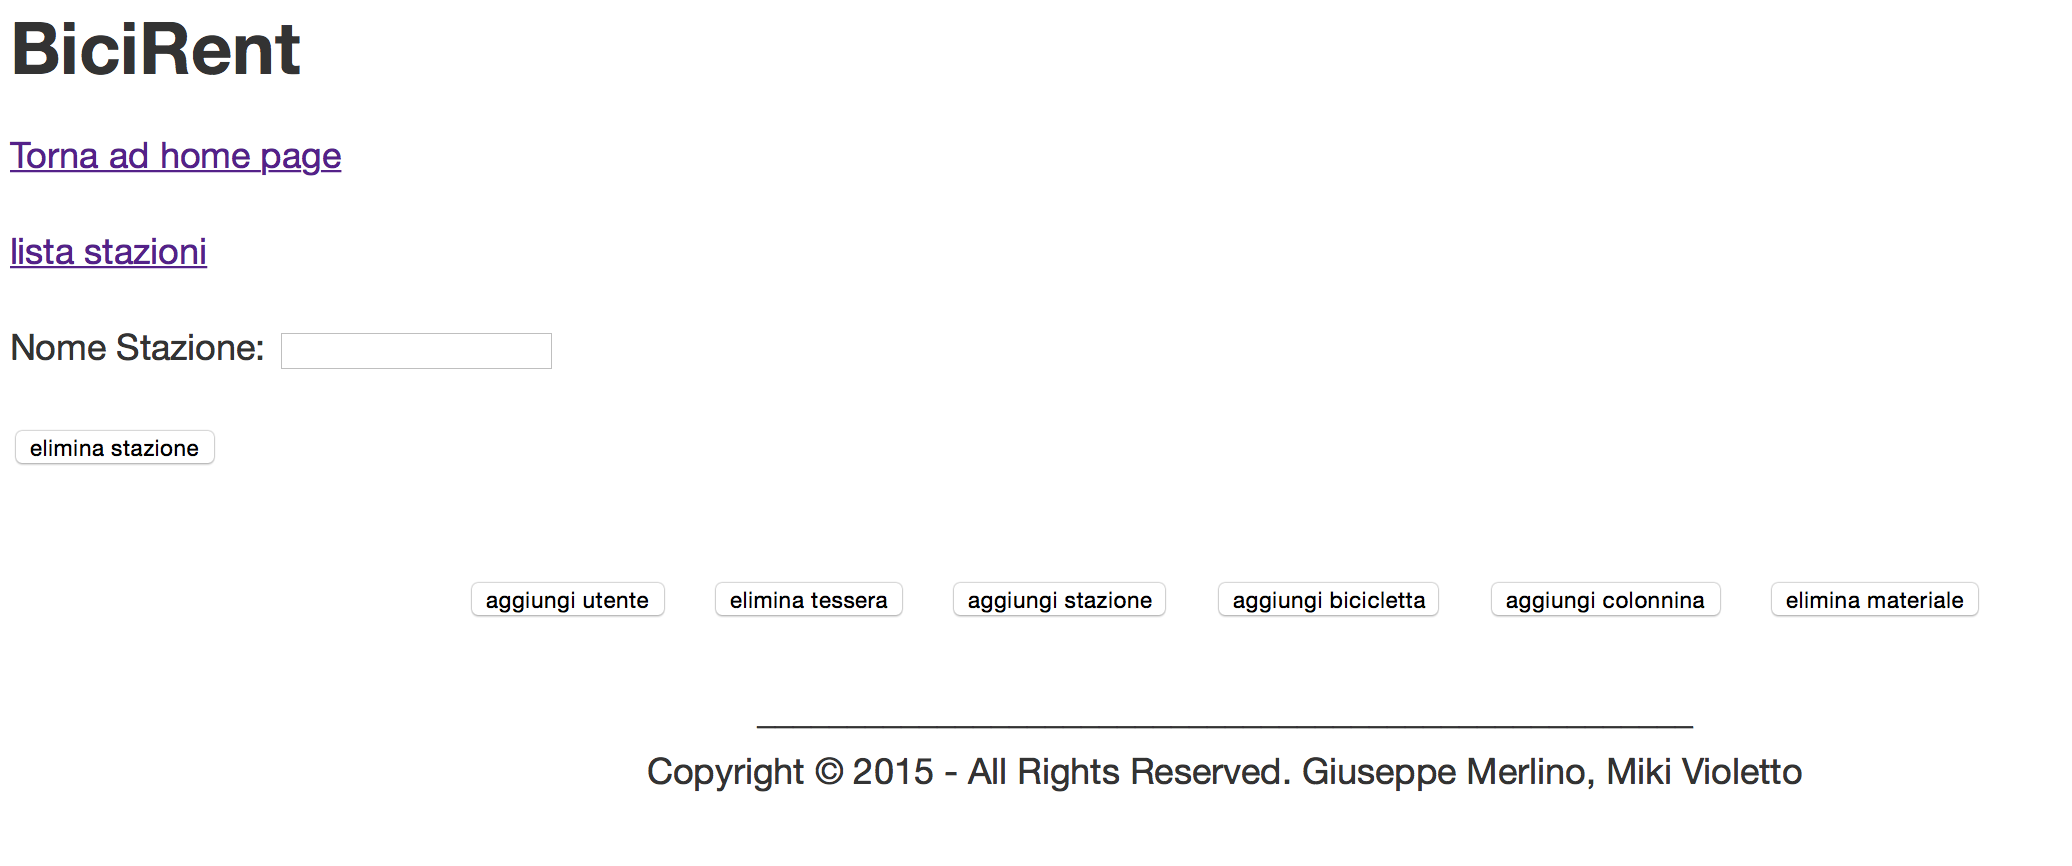
\includegraphics[width=0.8\textwidth]{Screenshot10}
	\caption{Rappresentazione admin.php?action=elimina+stazione}
\end{figure}
\subsubsection{Aggiungi bicicletta}
La form permette di inserire nel database una bicicletta e si presenta con una checkbox per indicare se essa sia elettrica o meno. Una volta terminato l'inserimento è possibile inviare la richiesta tramite il pulsante aggiungi bicicletta che ricaricherà la pagina e invierà i dati con metodo POST inserendo l'esito tramite GET nell'url. Inoltre è possibile consultare la lista biciclette cliccando l'apposito link.
\begin{figure}[H]
	\centering
	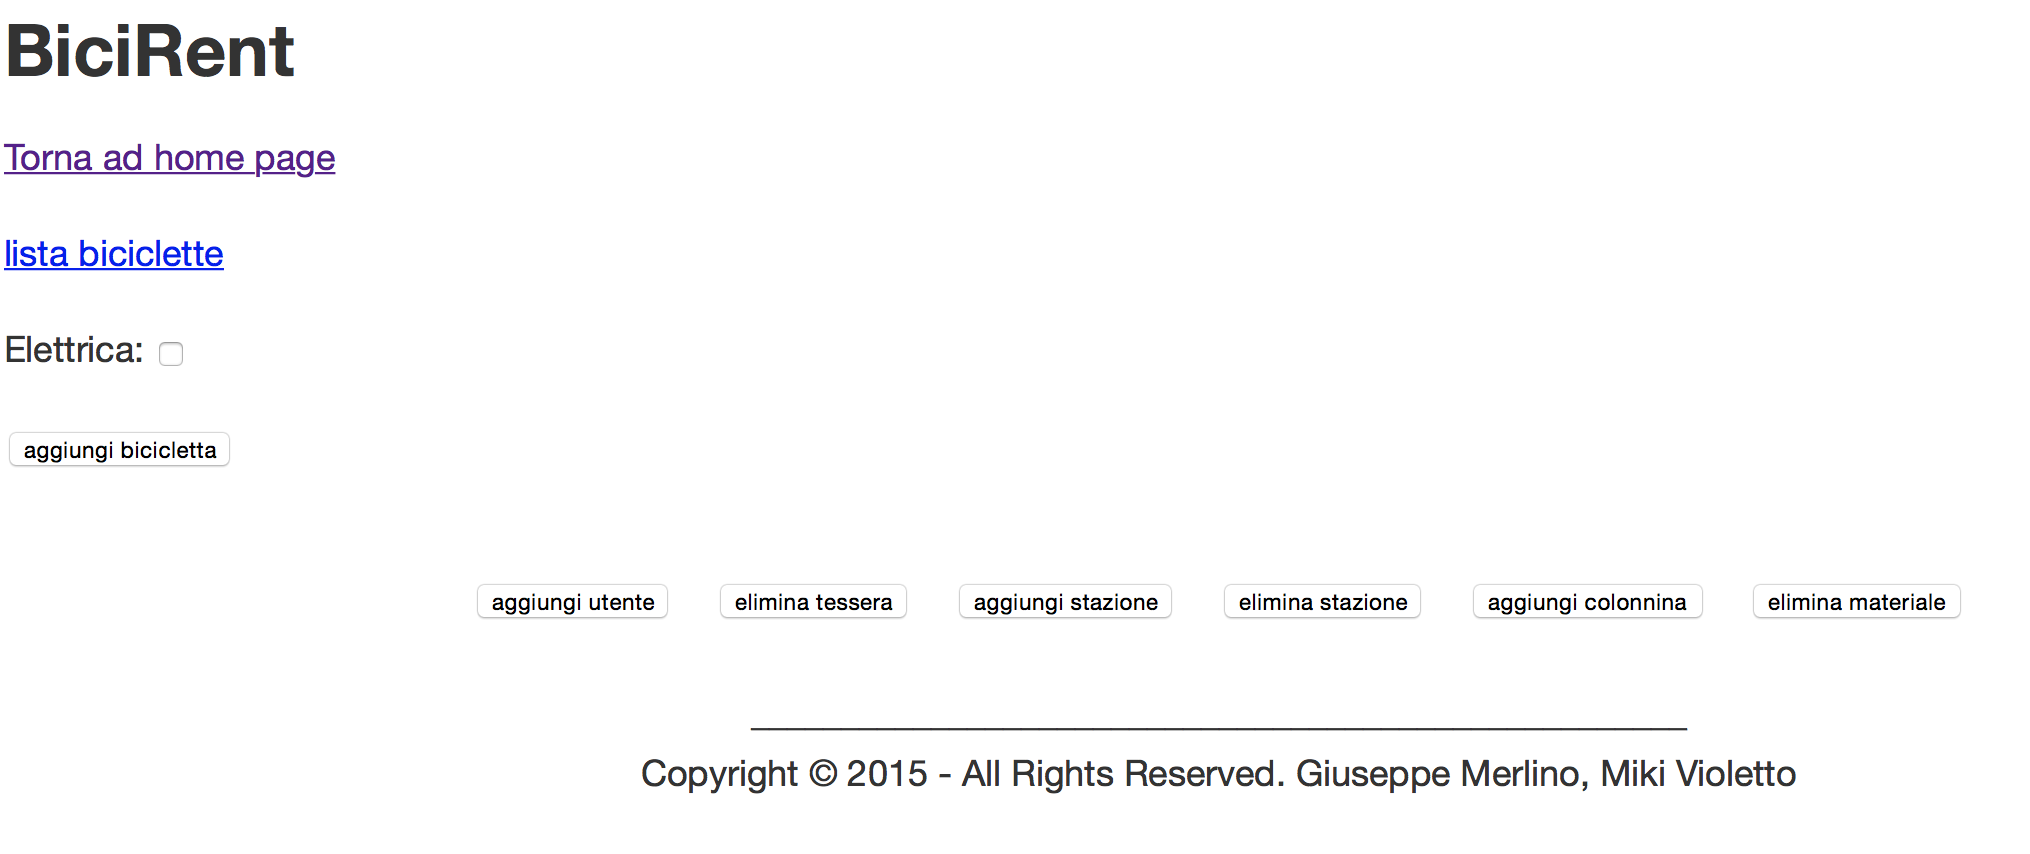
\includegraphics[width=0.8\textwidth]{Screenshot11}
	\caption{Rappresentazione admin.php?action=aggiungi+bicicletta}
\end{figure}
\subsubsection{Aggiungi colonnina}
La form permette di inserire nel database una colonnina e si presenta con un campo di testo per indicare la stazione a cui dovrà appartenere. Una volta terminato l'inserimento è possibile inviare la richiesta tramite il pulsante aggiungi colonnina che ricaricherà la pagina e invierà i dati con metodo POST inserendo l'esito tramite GET nell'url. Inoltre è possibile consultare la lista colonnine e quella delle stazioni cliccando gli appositi link.
\begin{figure}[H]
	\centering
	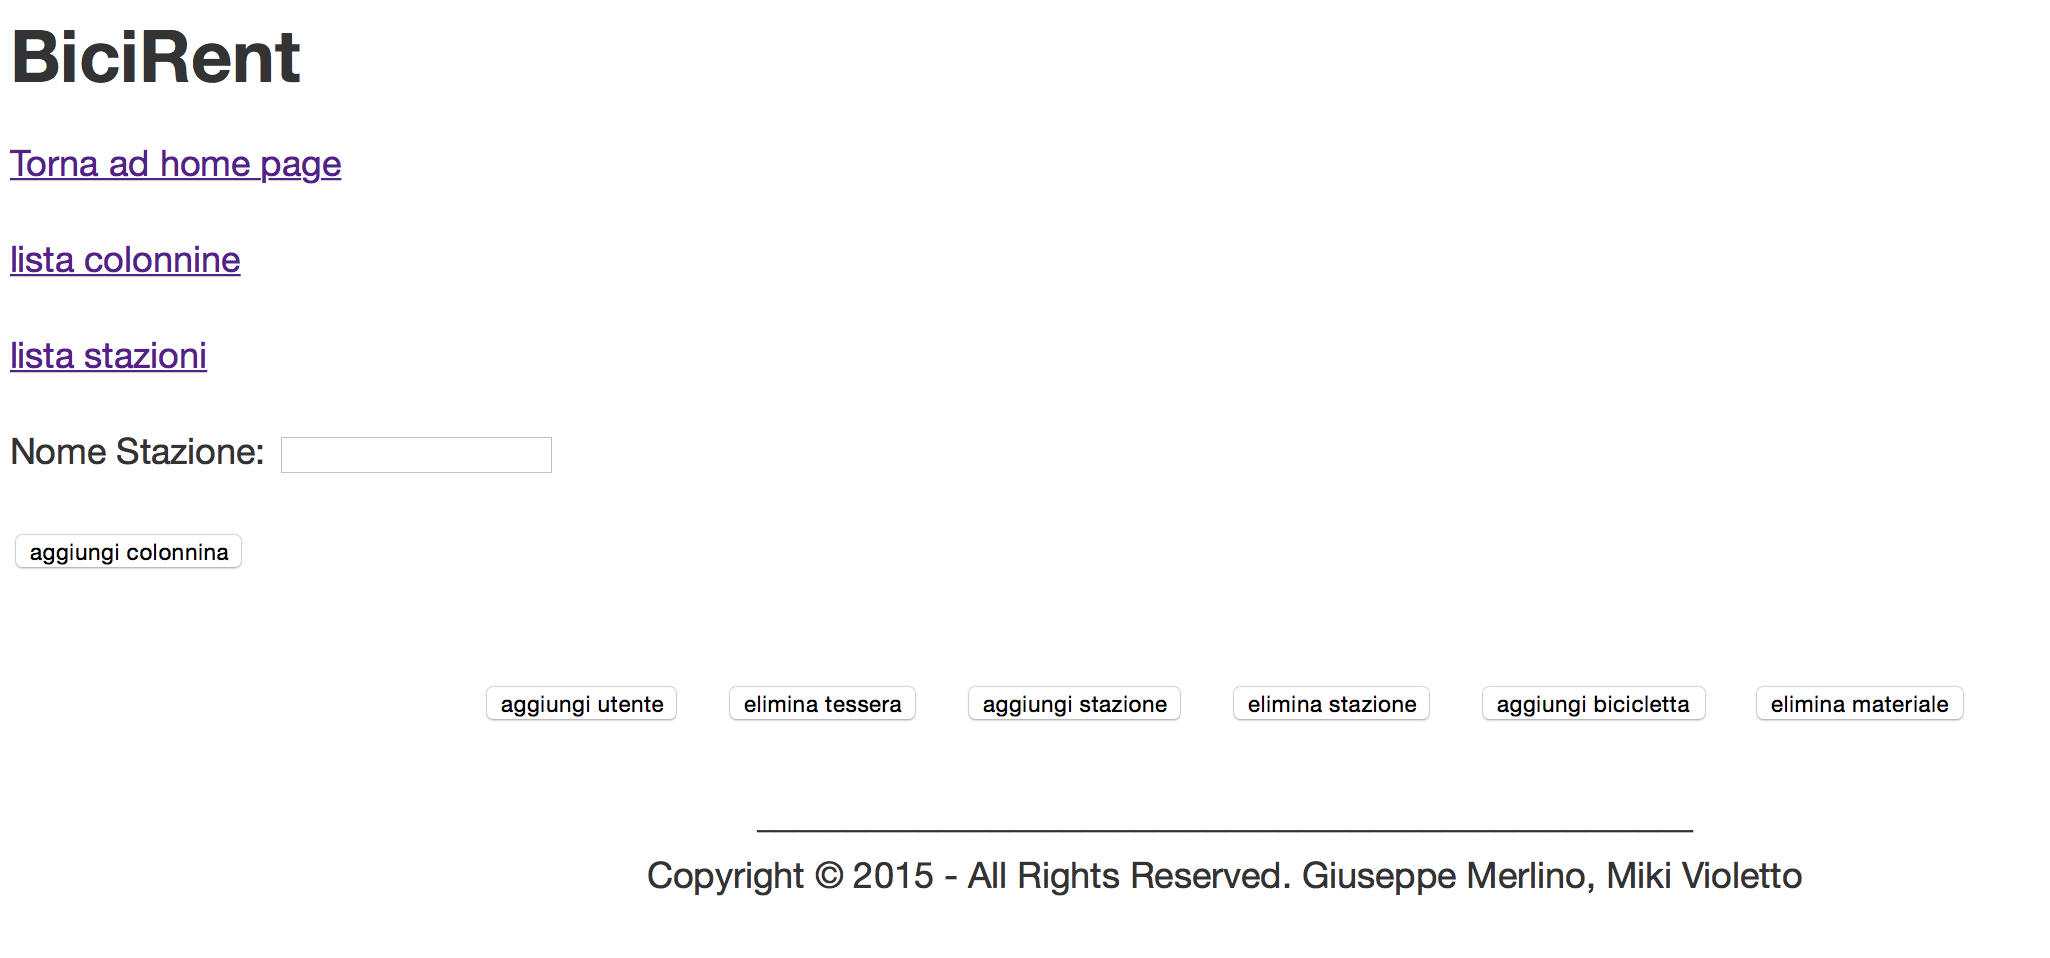
\includegraphics[width=0.8\textwidth]{Screenshot12}
	\caption{Rappresentazione admin.php?action=aggiungi+colonnina}
\end{figure}
\subsubsection{Elimina materiale}
La form permette di eliminare dal database una bicicletta o colonnina e si presenta con un campo di testo per indicare il codice materiale da eliminare. Una volta terminato l'inserimento è possibile inviare la richiesta tramite il pulsante elimina materiale che ricaricherà la pagina e invierà i dati con metodo POST inserendo l'esito tramite GET nell'url. Inoltre è possibile consultare la lista materiale cliccando l'apposito link.
\begin{figure}[H]
	\centering
	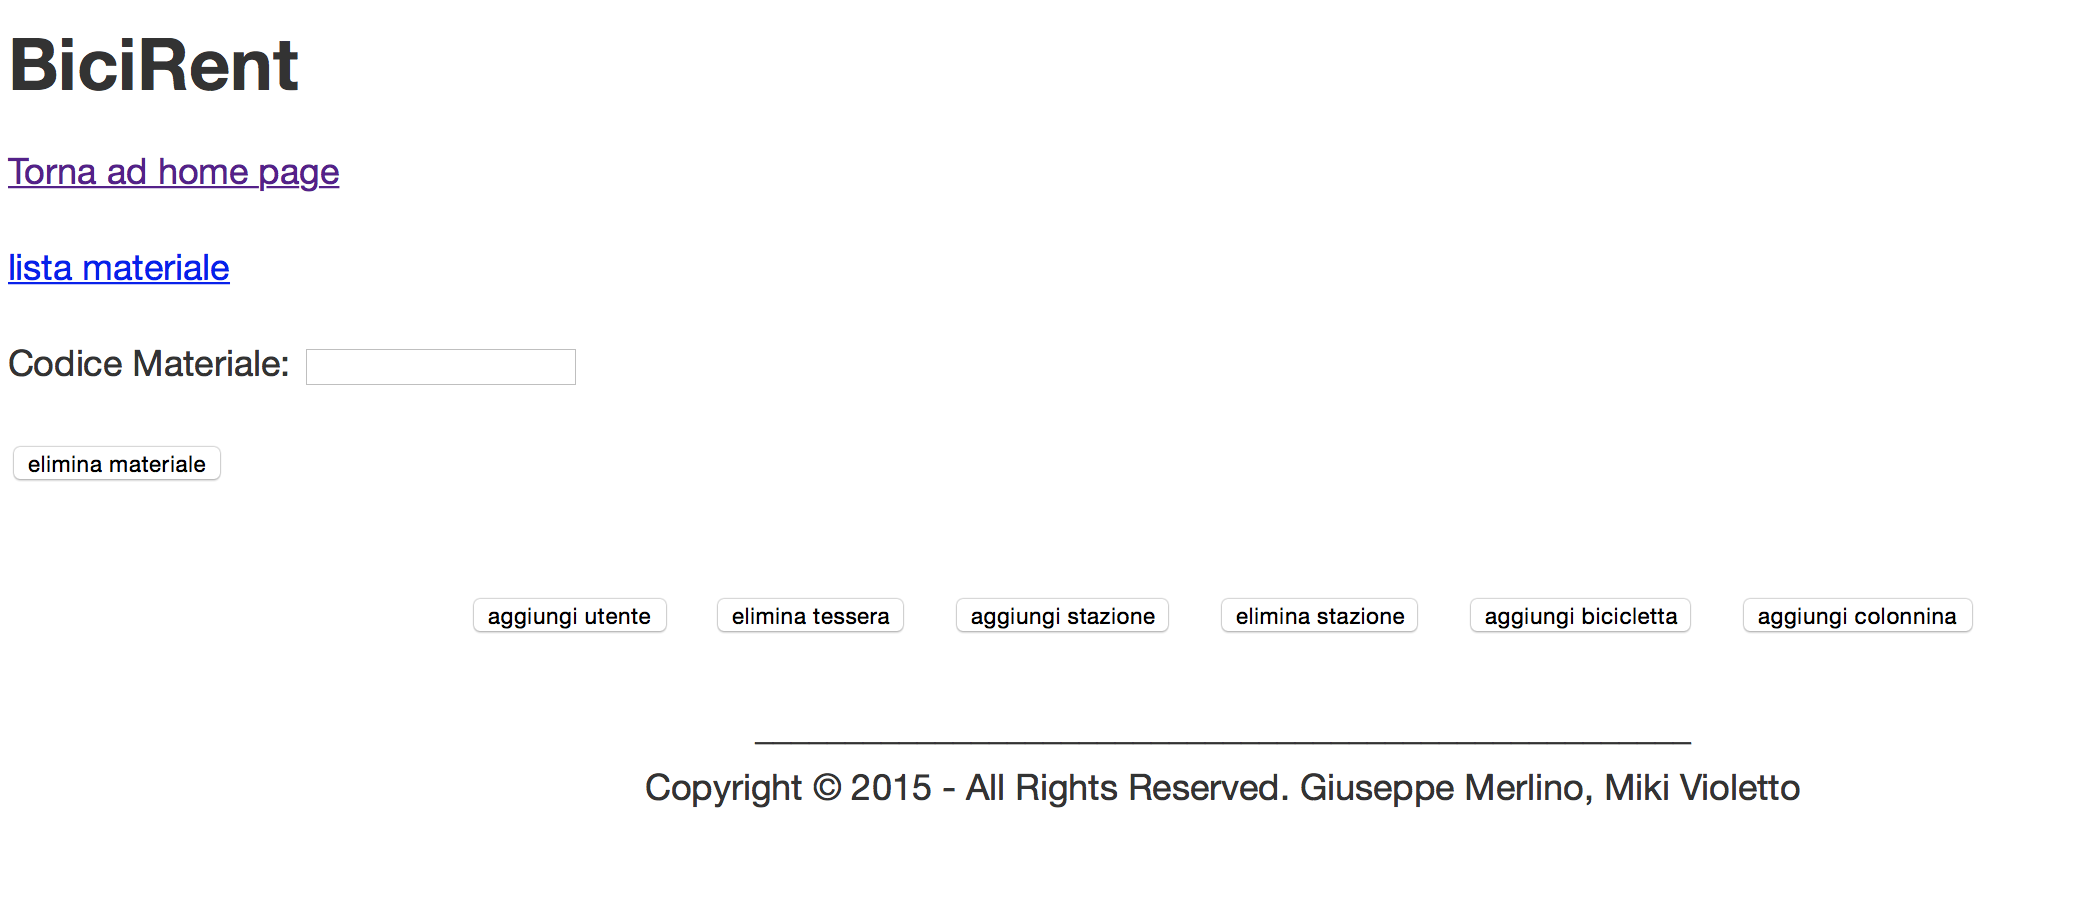
\includegraphics[width=0.8\textwidth]{Screenshot13}
	\caption{Rappresentazione admin.php?action=elimina+materiale}
\end{figure}
\subsubsection{Liste dell'area amministrativa}
I link che mostrano le liste di oggetti nelle sotto-sezioni dell'area amministrativa vengono indirizzati alla pagina mostra.php che tramite GET crea liste contenenti gli oggetti richiesti dalla rispettiva pagina admin.php.
\begin{figure}[H]
	\centering
	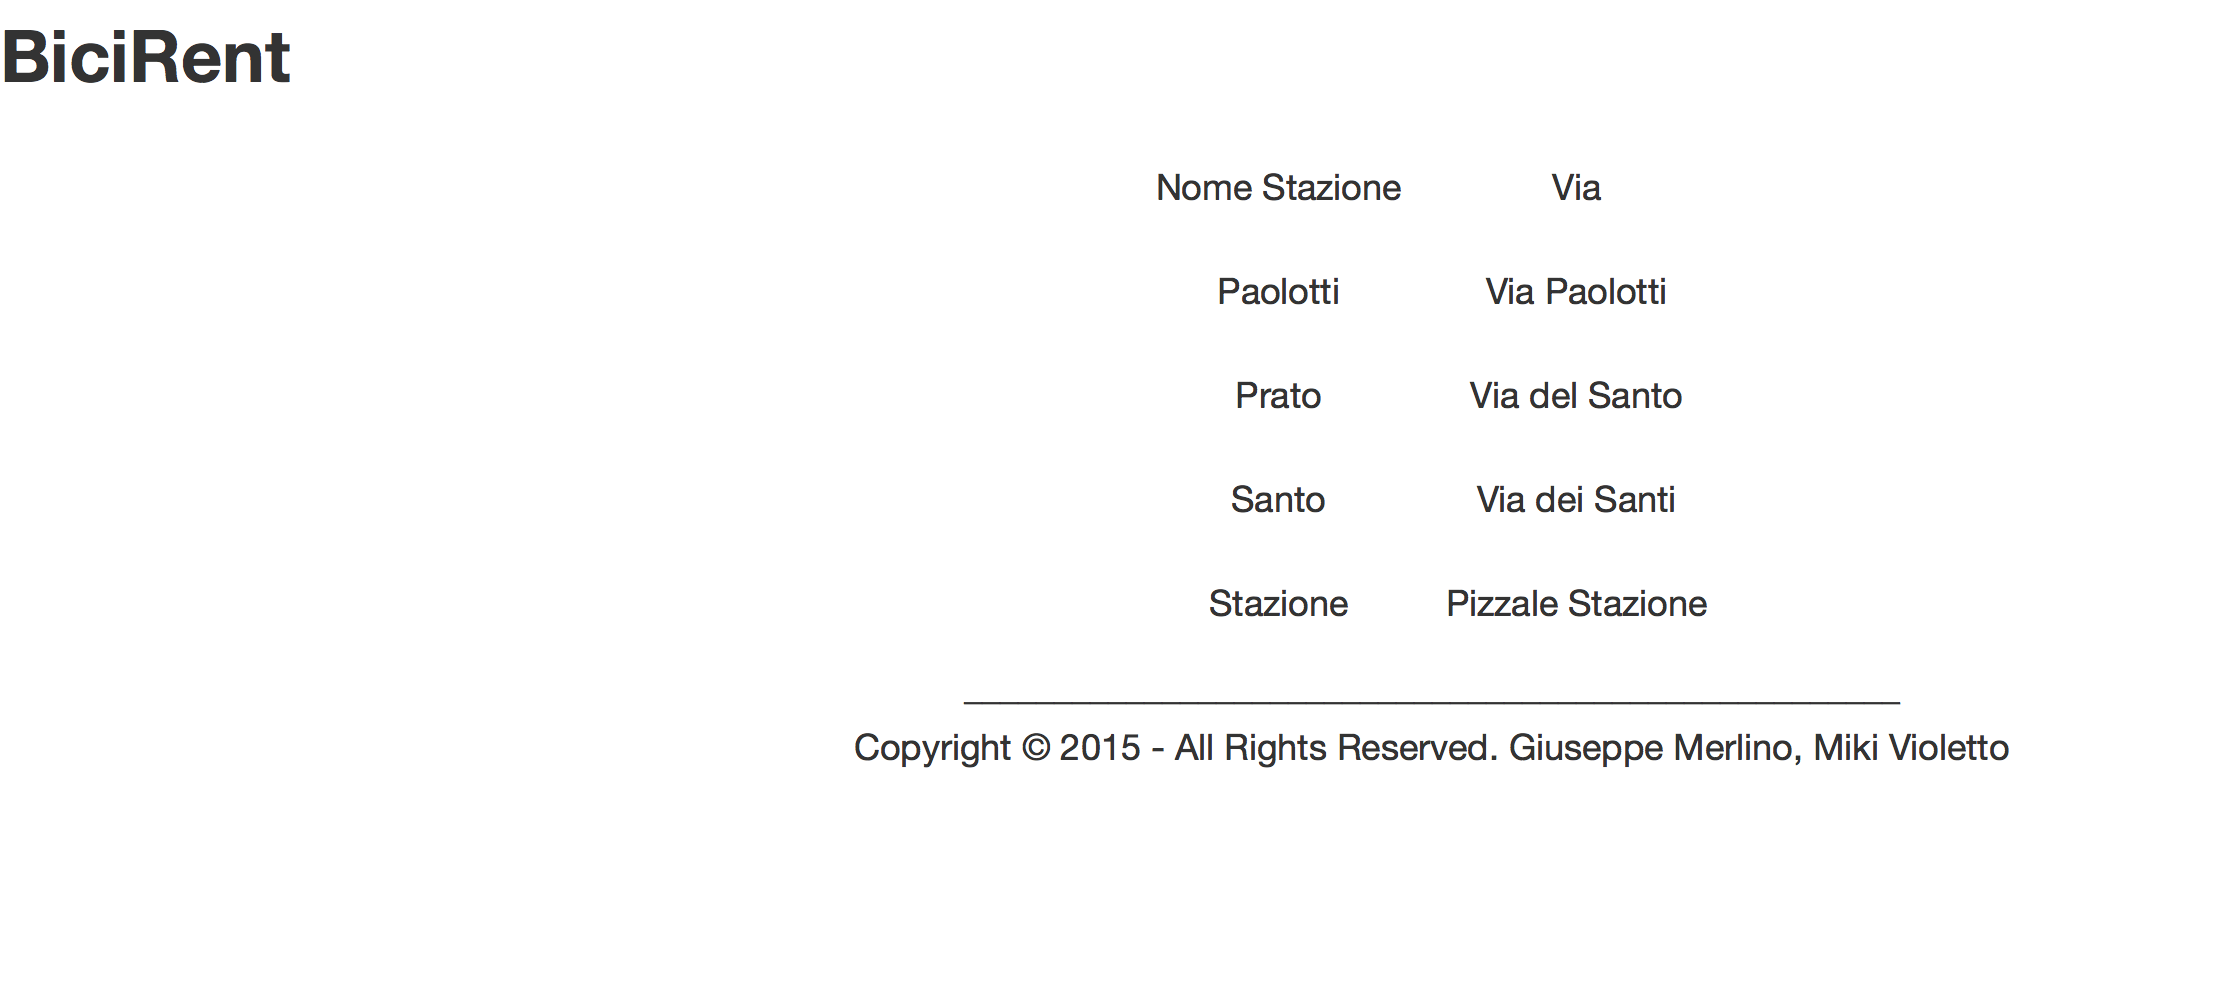
\includegraphics[width=0.8\textwidth]{Screenshot14}
	\caption{Rappresentazione mostra.php?action=stazione}
\end{figure}
\section{Conclusioni}
Il progetto si è rivelato estremamente interessante sia dal punto di vista pratico che didattico, inoltre abbiamo avuto la possibilità di utilizzare tecnologie come HTML, JavaScript, PHP, e MySQL insieme ottenendo risultati davvero eccezionali. Abbiamo inoltre cercato di curare il più possibile la facilità d'uso nell'esperienza utente con particolare attenzione agli errori e possibili fallback del sistema. Infine speriamo di aver riportato in maniera chiara tramite la seguente documentazione il lavoro svolto.
\end{document}